\documentclass{article}
\usepackage{amsmath}
\usepackage{amssymb}
\usepackage{geometry}
\usepackage{tikz}
\usepackage{booktabs}
\usepackage{array}
\newcolumntype{L}[1]{>{\raggedright\arraybackslash}p{#1}}
\usetikzlibrary{calc}
\geometry{a4paper, margin=1in}

\title{Digitized Notes - Image Processing}
\author{Aung Naing Oo}
\date{\today}

\begin{document}

\maketitle

% --- Left Page Content ---
\subsection*{Grid and Coordinate System}

The notes show a grid with coordinates labeled $x_1$ through $x_5$ horizontally and $y_1$ through $y_5$ vertically.

\begin{center}
\begin{tabular}{|c|c|c|c|c|c|}
\hline
& $y_1$ & $y_2$ & $y_3$ & $y_4$ & $y_5$ \\
\hline
$x_1$ & & & & & \\
\hline
$x_2$ & & & & & \\
\hline
$x_3$ & & & & & \\
\hline
$x_4$ & & & & & \\
\hline
$x_5$ & & & & & \\
\hline
\end{tabular}
\end{center}

\begin{itemize}
    \item Coordinate points would be for example ($x_3$, $y_2$), ($x_1$, $y_5$), etc.
    
\end{itemize}
\begin{center}
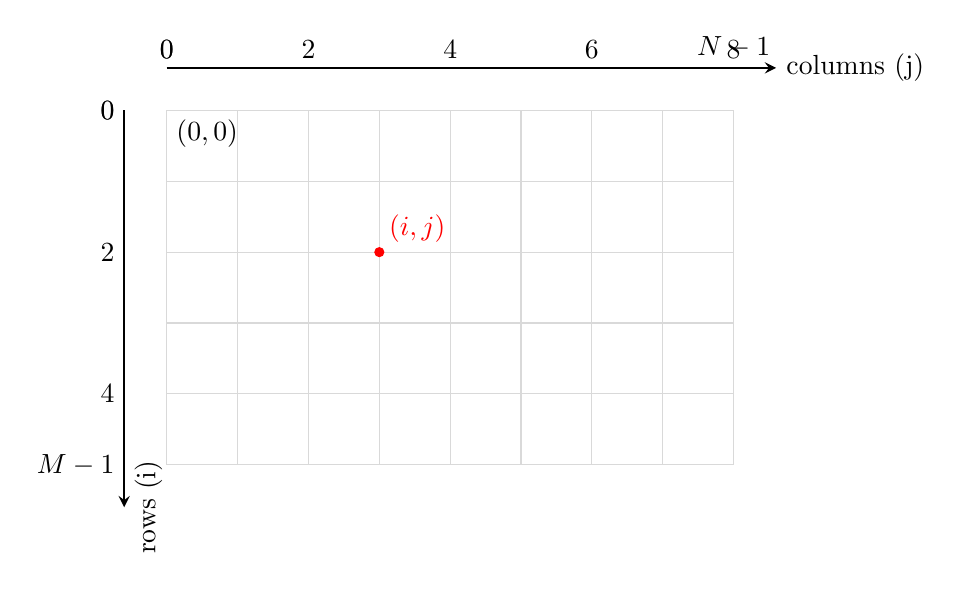
\begin{tikzpicture}[scale=0.9,>=stealth]
    % drawing size (for illustration only)
    \def\Cols{8} % visual columns (represents 0 .. N-1)
    \def\Rows{5} % visual rows (represents 0 .. M-1)

    % grid: columns to the right, rows downwards
    \draw[step=1cm,gray!30] (0,0) grid (\Cols,-\Rows);

    % top horizontal axis (columns)
    \draw[->,thick] (0,0.6) -- (\Cols+0.6,0.6) node[right] {columns (j)};
    \node[above] at (0,0.6) {0};
    \node[above] at (\Cols,0.6) {$N-1$};

    % left vertical axis (rows) pointing downward
    \draw[->,thick] (-0.6,0) -- (-0.6,-\Rows-0.6) node[below,rotate=90] {rows (i)};
    \node[left] at (-0.6,0) {0};
    \node[left] at (-0.6,-\Rows) {$M-1$};

    % origin label at top-left
    \node[anchor=north west] at (0,0) {$(0,0)$};

    % example point (i,j) shown inside grid
    \coordinate (p) at (3,-2);
    \filldraw[red] (p) circle (1.8pt) node[above right] {$(i,j)$};

    % optional tick labels along top and left for clarity
    \foreach \x in {0,2,4,6,8} \node[above] at (\x,0.6) {\x};
    \foreach \y in {0,2,4} \node[left] at (-0.6,-\y) {\y};
\end{tikzpicture}
\end{center}


\subsubsection*{Binary Representation}
\begin{itemize}
    \item $0 \to \text{black}$
    \item $1 \to \text{white}$
\end{itemize}

\begin{center}
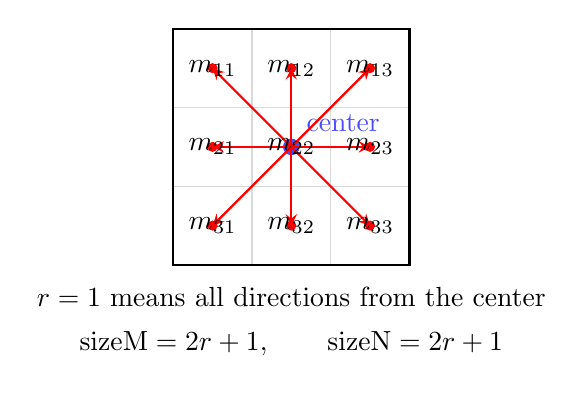
\begin{tikzpicture}[scale=1,>=stealth]
    % 3x3 grid
    \draw[step=1cm,gray!30] (0,0) grid (3,3);
    \draw[thick] (0,0) rectangle (3,3);

    % center coordinate
    \coordinate (c) at (1.5,1.5);
    \filldraw[blue!70] (c) circle (2.8pt) node[above right,xshift=2pt,yshift=2pt] {center};

    % arrows from center to all neighbor directions (8-neighborhood)
    \foreach \dx/\dy in {-1/1,0/1,1/1,-1/0,1/0,-1/-1,0/-1,1/-1}{
        \draw[->,red,thick] (c) -- ($(c)+(\dx,\dy)$);
        \filldraw[red] ($(c)+(\dx,\dy)$) circle (1.6pt);
    }

    % optional small matrix labels (optional)
    \node at (0.5,2.5) {$m_{11}$};
    \node at (1.5,2.5) {$m_{12}$};
    \node at (2.5,2.5) {$m_{13}$};
    \node at (0.5,1.5) {$m_{21}$};
    \node at (1.5,1.5) {$m_{22}$};
    \node at (2.5,1.5) {$m_{23}$};
    \node at (0.5,0.5) {$m_{31}$};
    \node at (1.5,0.5) {$m_{32}$};
    \node at (2.5,0.5) {$m_{33}$};

    % explanatory labels
    \node at (1.5,-0.4) {$r=1\ \text{means all directions from the center}$};
    \node at (1.5,-1.0) {$\mathrm{sizeM}=2r+1,\qquad \mathrm{sizeN}=2r+1$};
\end{tikzpicture}
\end{center}



% --- Right Page Content ---

\subsubsection*{General Reminder}
Need to remember the **grid format** and **coordinate system**.

\subsubsection*{Clipping/Normalization Formula}
The formula for normalization (or scaling/clipping) of a function $f(x,y)$ to the range $[0, 255]$ is noted:
$$
g(x,y) \to 255 \cdot \frac{f(x,y) - \min}{\max - \min}
$$
\begin{itemize}
    \item $f(x,y)$ is the original intensity value at $(x,y)$.
    \item $\min$ and $\max$ are the minimum and maximum intensity values in the image.
\end{itemize}

\begin{verbatim}
rescaledNebulaNoisy = 255*(noisy - Min[noisy])/(Max[noisy] - Min[noisy]);
rescaledNebulaNoisy = Rescale[noisy, MinMax@noisy, {0,255}];
\end{verbatim}



\subsubsection*{Intensity Transformation}
The general form for an intensity transformation where $f(x,y)$ is the input image and $g(x,y)$ is the output image using a transformation $T$:
$$
g(x,y) = T[f(x,y)]
$$

\subsubsection*{Thresholding}
\textbf{Thresholding} is the process of producing a **binary image** (2 levels of intensity, e.g., 0 and 1 or black and white).

\begin{itemize}
    \item The thresholding operation can be visualized as:
    \begin{center}
    \begin{tikzpicture}[scale=1.1]
        % Axes
        \draw[->] (0,0) -- (5.5,0) node[right] {$f(x,y)$};
        \draw[->] (0,0) -- (0,3.2) node[above] {$g(x,y)$};

        % Threshold line at k
        \draw[dashed] (2,0) -- (2,2.5);
        \node[below] at (2,0) {$k$};

        % Flat region below k
        \draw[thick,blue] (0,0) -- (2,0);

        % Step up to 255 at k
        \draw[thick,blue] (2,0) -- (2,2.5);
        \draw[thick,blue] (2,2.5) -- (5,2.5);

        % 255 label
        \node[left] at (0,2.5) {$255$};

        % Function label
        \node[above right,blue] at (3.5,2.5) {$g(x,y)$};

        % Add sample points
        \foreach \x in {0.5,1,1.5}
            \filldraw[blue] (\x,0) circle (1.2pt);
        \foreach \x in {2.5,3,4.5}
            \filldraw[blue] (\x,2.5) circle (1.2pt);
    \end{tikzpicture}
    \end{center}
    \item The thresholding function is:
    \[
    g(x,y) =
    \begin{cases}
    0, & f(x,y) < k \\
    255, & f(x,y) \geq k
    \end{cases}
    \]
    
\end{itemize}

\subsubsection*{How the Threshold Works}

The function processes the input image $\text{img}$ and applies the following rule to each pixel's intensity value:

\begin{itemize}
    \item If the pixel's intensity is less than threshold value, the resulting binary pixel is set to black (intensity 0).
    \item If the pixel's intensity is greater than the threshold value, the resulting binary pixel is set to white (intensity 1, or maximum).
\end{itemize}

\textbf{Example in Mathematica:}
\begin{verbatim}
Binarize[lowPassFiltered, 0.2]
\end{verbatim}




\subsection*{Log Transformation}
Log transformation is used to expand dark pixel values in an image while compressing higher intensity values. The general formula is:
\[
g(x,y) = c \cdot \log\left(1 + f(x,y)\right)
\]
where:
\begin{itemize}
    \item $f(x,y)$ is the input pixel value.
    \item $g(x,y)$ is the output pixel value.
    \item $c$ is a scaling constant, often chosen so that the maximum output value is 255.
\end{itemize}

\subsubsection*{Finding the Constant $c$}
When $g(x,y) = 255$ and $f(x,y) = 255$:
\[
255 = c \cdot \log(1 + 255)
\]
\[
c = \frac{255}{\log(256)}
\]
\begin{center}
\begin{tikzpicture}[scale=1.1]
    % Axes
    \draw[->] (0,0) -- (5.5,0) node[right] {$f(x,y)$};
    \draw[->] (0,0) -- (0,3.2) node[above] {$g(x,y)$};

    % Log curve
    \draw[thick,blue,domain=0:5,samples=60] plot (\x,{2.5*ln(1+\x)/ln(6)});
    \node[above right,blue] at (4,2.1) {$g(x,y) = c \cdot \log(1 + f(x,y))$};

    % 255 label
    \node[left] at (0,2.5) {$255$};
\end{tikzpicture}
\end{center}


\subsection*{Reversing Intensity Levels}
Reversing (or inverting) the intensity levels of an image produces a **negative** image. The formula is:
\[
g(x,y) = (L - 1) - f(x,y)
\]
where:
\begin{itemize}
    \item $f(x,y)$ is the input pixel value.
    \item $g(x,y)$ is the output pixel value (inverted).
    \item $L$ is the number of intensity levels (e.g., 256 for an 8-bit image, so $L-1 = 255$).
\end{itemize}

\subsubsection*{Example}
For an 8-bit image ($L = 256$):
\[
g(x,y) = 255 - f(x,y)
\]
This transformation maps dark pixels to bright pixels and vice versa.

\begin{center}
\begin{tikzpicture}[scale=1.1]
    % Axes
    \draw[->] (0,0) -- (5.5,0) node[right] {$f(x,y)$};
    \draw[->] (0,0) -- (0,3.2) node[above] {$g(x,y)$};

    % Inversion line
    \draw[thick,blue] (0,2.5) -- (5,0);
    \node[above right,blue] at (4,0.8) {$g(x,y) = (L-1) - f(x,y)$};

    % 255 label
    \node[left] at (0,2.5) {$255$};
    \node[below] at (5,0) {$255$};
\end{tikzpicture}
\end{center}

\subsection*{Power Law Transformation}
Power law transformation is used to enhance image contrast by applying a nonlinear transformation. The general formula is:
\[
g(x,y) = c \cdot [f(x,y)]^{\gamma}
\]
where:
\begin{itemize}
    \item $f(x,y)$ is the input pixel value.
    \item $g(x,y)$ is the output pixel value.
    \item $c$ is a scaling constant.
    \item $\gamma$ (gamma) is the exponent that controls the transformation:
    \begin{itemize}
        \item $\gamma > 1$ brightens the image (expands dark values).
        \item $\gamma < 1$ darkens the image (compresses bright values).
        \item $\gamma = 1$ produces a linear transformation.
    \end{itemize}
\end{itemize}


\subsection*{Power Law Transformation - Multiple Gamma Values}
The following figure shows how different gamma values affect the intensity transformation:

\begin{center}
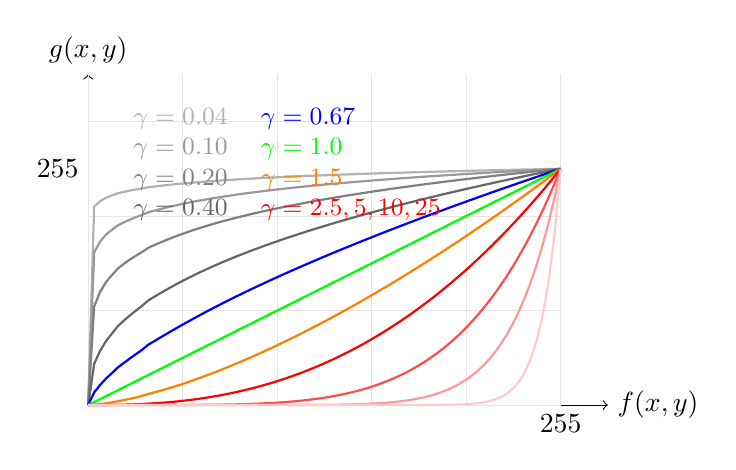
\begin{tikzpicture}[scale=1.2]
    % Axes
    \draw[->] (0,0) -- (5.5,0) node[right] {$f(x,y)$};
    \draw[->] (0,0) -- (0,3.5) node[above] {$g(x,y)$};

    % Grid
    \draw[step=1,gray!20] (0,0) grid (5,3.5);

    % Diagonal reference line (gamma = 1)
    \draw[thick,gray!50,dashed] (0,0) -- (5,2.5);

    % Power law curves for different gamma values
    \draw[thick,black!30,domain=0:5,samples=80] plot (\x,{2.5*(\x/5)^0.04});
    \draw[thick,black!40,domain=0:5,samples=80] plot (\x,{2.5*(\x/5)^0.10});
    \draw[thick,black!50,domain=0:5,samples=80] plot (\x,{2.5*(\x/5)^0.20});
    \draw[thick,black!60,domain=0:5,samples=80] plot (\x,{2.5*(\x/5)^0.40});
    \draw[thick,blue,domain=0:5,samples=80] plot (\x,{2.5*(\x/5)^0.67});
    \draw[thick,green,domain=0:5,samples=80] plot (\x,{2.5*(\x/5)^1.0});
    \draw[thick,orange,domain=0:5,samples=80] plot (\x,{2.5*(\x/5)^1.5});
    \draw[thick,red,domain=0:5,samples=80] plot (\x,{2.5*(\x/5)^2.5});
    \draw[thick,red!70,domain=0:5,samples=80] plot (\x,{2.5*(\x/5)^5});
    \draw[thick,red!40,domain=0:5,samples=80] plot (\x,{2.5*(\x/5)^10});
    \draw[thick,red!20,domain=0:5,samples=80] plot (\x,{2.5*(\x/5)^25});

    % Labels
    \node[left] at (0,2.5) {$255$};
    \node[below] at (5,0) {$255$};

    % Legend
    \node[anchor=north west,font=\small] at (0.2,3.3) {
        \begin{tabular}{ll}
        \textcolor{black!30}{$\gamma=0.04$} & \textcolor{blue}{$\gamma=0.67$} \\
        \textcolor{black!40}{$\gamma=0.10$} & \textcolor{green}{$\gamma=1.0$} \\
        \textcolor{black!50}{$\gamma=0.20$} & \textcolor{orange}{$\gamma=1.5$} \\
        \textcolor{black!60}{$\gamma=0.40$} & \textcolor{red}{$\gamma=2.5, 5, 10, 25$}
        \end{tabular}
    };
\end{tikzpicture}
\end{center}

Observations:
\begin{itemize}
    \item For $\gamma < 1$: curves are above the diagonal, brightening the image.
    \item For $\gamma = 1$: linear transformation (diagonal line).
    \item For $\gamma > 1$: curves are below the diagonal, darkening the image and increasing contrast in bright regions.
    \item As $\gamma$ increases, the compression of bright values becomes more pronounced.
\end{itemize}

\subsection*{Contrast Stretching}
Contrast stretching is a technique used to expand the range of intensity levels in an image. It uses a piecewise linear transformation to map input intensity levels to output levels.

\subsubsection*{Piecewise Linear Transformation}
The transformation is defined by two control points $(r_1, s_1)$ and $(r_2, s_2)$:

\[
g(x,y) = \begin{cases}
\frac{s_1}{r_1} \cdot f(x,y), & f(x,y) < r_1 \\
\frac{s_2 - s_1}{r_2 - r_1} \cdot (f(x,y) - r_1) + s_1, & r_1 \leq f(x,y) \leq r_2 \\
\frac{255 - s_2}{255 - r_2} \cdot (f(x,y) - r_2) + s_2, & f(x,y) > r_2
\end{cases}
\]

\subsubsection*{Example with Given Values}
For $r_1 = 9$, $s_1 = 10$, $r_2 = 80$, and $s_2 = 90$:

\begin{center}
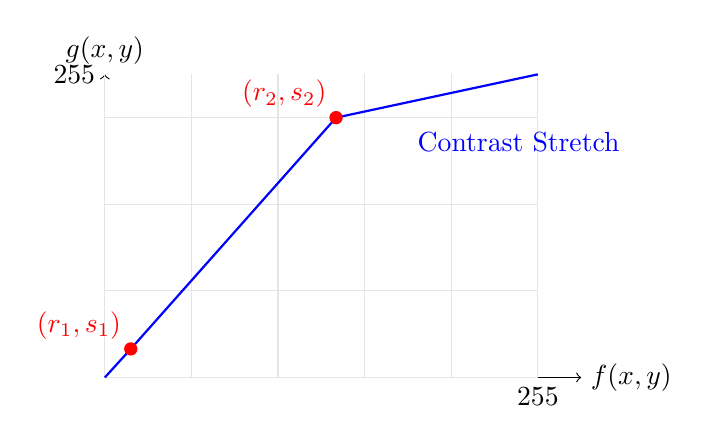
\begin{tikzpicture}[scale=1.1]
    % Axes
    \draw[->] (0,0) -- (5.5,0) node[right] {$f(x,y)$};
    \draw[->] (0,0) -- (0,3.5) node[above] {$g(x,y)$};

    % Grid
    \draw[step=1,gray!20] (0,0) grid (5,3.5);

    % Calculate coordinates for control points
    % r1=9, s1=10, r2=80, s2=90 (scaled to fit plot: divide by ~30)
    % r1 -> ~0.3, s1 -> ~0.33, r2 -> ~2.67, s2 -> ~3
    
    % Piecewise linear transformation
    \draw[thick,blue] (0,0) -- (0.3,0.33);
    \draw[thick,blue] (0.3,0.33) -- (2.67,3);
    \draw[thick,blue] (2.67,3) -- (5,3.5);

    % Mark control points
    \filldraw[red] (0.3,0.33) circle (2pt) node[above left] {$(r_1, s_1)$};
    \filldraw[red] (2.67,3) circle (2pt) node[above left] {$(r_2, s_2)$};

    % Labels
    \node[left] at (0,3.5) {$255$};
    \node[below] at (5,0) {$255$};
    \node[above right,blue] at (3.5,2.5) {Contrast Stretch};
\end{tikzpicture}
\end{center}

\begin{itemize}
    \item Intensities below $r_1 = 9$ are compressed to $[0, s_1]$.
    \item Intensities between $r_1$ and $r_2$ are stretched to $[s_1, s_2]$.
    \item Intensities above $r_2 = 80$ are stretched to $[s_2, 255]$.
    \item This expands the dynamic range and increases contrast.
\end{itemize}


\subsection*{Intensity Level Slicing}
Intensity level slicing is a technique used to highlight specific ranges of intensity values in an image while suppressing others. This method is particularly useful for emphasizing certain features or objects within an image.

\subsubsection*{Definition}
The intensity level slicing operation can be defined as follows:
\[
g(x,y) =
\begin{cases}
255, & \text{if } L_1 \leq f(x,y) \leq L_2 \\
0, & \text{otherwise}
\end{cases}
\]
where:
\begin{itemize}
    \item \( f(x,y) \) is the input pixel value.
    \item \( g(x,y) \) is the output pixel value.
    \item \( L_1 \) and \( L_2 \) are the lower and upper bounds of the intensity range to be highlighted.
\end{itemize}

\subsubsection*{Example}
For example, if we want to highlight intensity values between 100 and 150, the transformation would be:
\[
g(x,y) =
\begin{cases}
255, & \text{if } 100 \leq f(x,y) \leq 150 \\
0, & \text{otherwise}
\end{cases}
\]

\subsubsection*{Visualization}
The following figure illustrates the effect of intensity level slicing on an image:

\begin{center}
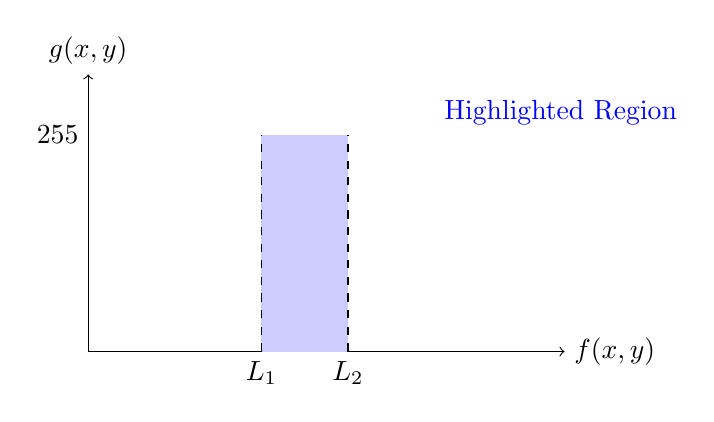
\begin{tikzpicture}[scale=1.1]
    % Axes
    \draw[->] (0,0) -- (5.5,0) node[right] {$f(x,y)$};
    \draw[->] (0,0) -- (0,3.2) node[above] {$g(x,y)$};

    % Highlighted region
    \fill[blue!20] (2,0) rectangle (3,2.5);
    
    % Threshold lines
    \draw[dashed] (2,0) -- (2,2.5);
    \draw[dashed] (3,0) -- (3,2.5);
    
    % Labels
    \node[below] at (2,0) {$L_1$};
    \node[below] at (3,0) {$L_2$};
    \node[above right,blue] at (4,2.5) {Highlighted Region};
    \node[left] at (0,2.5) {$255$};
\end{tikzpicture}
\end{center}

This technique effectively creates a binary image where only the specified intensity range is visible, enhancing the features of interest.

\newpage
\section*{Histogram Techniques}

\subsection*{Histogram Equalisation}


\begin{center}
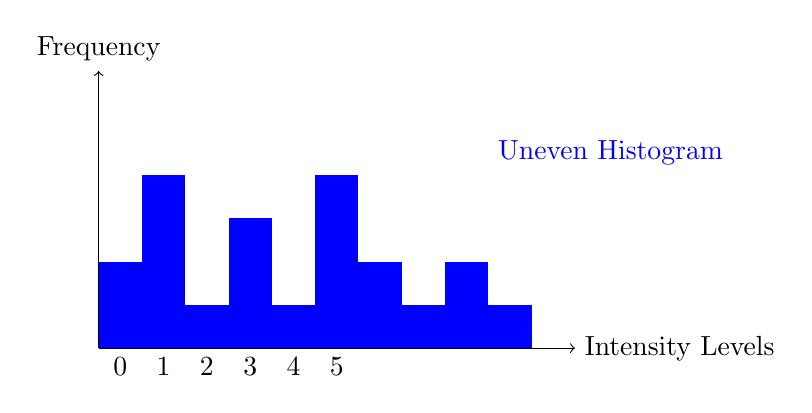
\begin{tikzpicture}[scale=1.1]
    % Axes
    \draw[->] (0,0) -- (5.5,0) node[right] {Intensity Levels};
    \draw[->] (0,0) -- (0,3.2) node[above] {Frequency};

    % Uneven histogram
    \fill[blue] (0,0) rectangle (0.5,1);
    \fill[blue] (0.5,0) rectangle (1,2);
    \fill[blue] (1,0) rectangle (1.5,0.5);
    \fill[blue] (1.5,0) rectangle (2,1.5);
    \fill[blue] (2,0) rectangle (2.5,0.5);
    \fill[blue] (2.5,0) rectangle (3,2);
    \fill[blue] (3,0) rectangle (3.5,1);
    \fill[blue] (3.5,0) rectangle (4,0.5);
    \fill[blue] (4,0) rectangle (4.5,1);
    \fill[blue] (4.5,0) rectangle (5,0.5);

    % Labels
    \node[below] at (0.25,0) {0};
    \node[below] at (0.75,0) {1};
    \node[below] at (1.25,0) {2};
    \node[below] at (1.75,0) {3};
    \node[below] at (2.25,0) {4};
    \node[below] at (2.75,0) {5};
    \node[above right,blue] at (4.5,2) {Uneven Histogram};
\end{tikzpicture}
\end{center}

\begin{center}
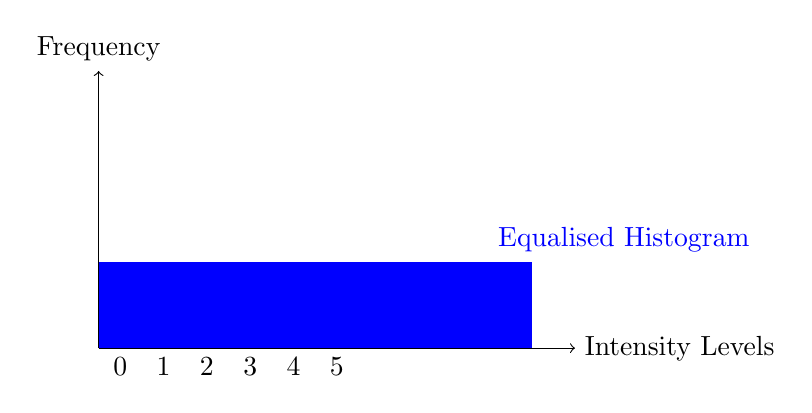
\begin{tikzpicture}[scale=1.1]
    % Axes
    \draw[->] (0,0) -- (5.5,0) node[right] {Intensity Levels};
    \draw[->] (0,0) -- (0,3.2) node[above] {Frequency};

    % Equalised histogram
    \fill[blue] (0,0) rectangle (0.5,1);
    \fill[blue] (0.5,0) rectangle (1,1);
    \fill[blue] (1,0) rectangle (1.5,1);
    \fill[blue] (1.5,0) rectangle (2,1);
    \fill[blue] (2,0) rectangle (2.5,1);
    \fill[blue] (2.5,0) rectangle (3,1);
    \fill[blue] (3,0) rectangle (3.5,1);
    \fill[blue] (3.5,0) rectangle (4,1);
    \fill[blue] (4,0) rectangle (4.5,1);
    \fill[blue] (4.5,0) rectangle (5,1);

    % Labels
    \node[below] at (0.25,0) {0};
    \node[below] at (0.75,0) {1};
    \node[below] at (1.25,0) {2};
    \node[below] at (1.75,0) {3};
    \node[below] at (2.25,0) {4};
    \node[below] at (2.75,0) {5};
    \node[above right,blue] at (4.5,1) {Equalised Histogram};
\end{tikzpicture}
\end{center}

\begin{center}
\textit{Histogram equalisation makes the histogram of an image as linear as possible.}
\end{center}

\subsection*{Histogram Matching}
Histogram matching transforms the histogram of the original image to a specific histogram we wish the original image to possess. This technique is useful for adjusting the brightness and contrast of an image to match a desired reference image.

\subsection*{Local Histogram Processing}

\begin{center}
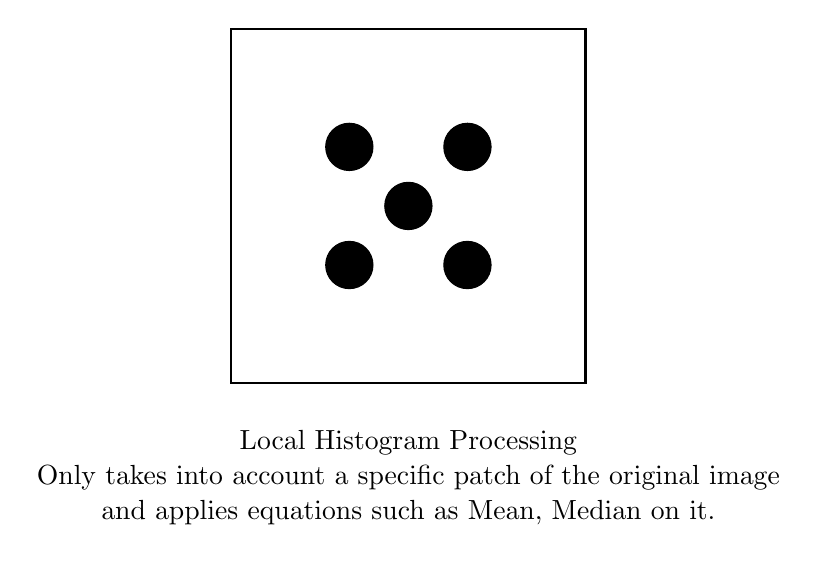
\begin{tikzpicture}[scale=1.5]
    % Draw the outline of the dice
    \draw[thick] (0,0) rectangle (3,3);
    
    % Draw the dots on the dice
    \foreach \x/\y in {1/1, 2/2, 1/2, 2/1, 1.5/1.5} {
        \filldraw[black] (\x,\y) circle (0.2);
    }

  
    % Add a label
    \node at (1.5,-0.5) {Local Histogram Processing};
    \node at (1.5,-0.8) {Only takes into account a specific patch of the original image};
    \node at (1.5,-1.1) {and applies equations such as Mean, Median on it.};
\end{tikzpicture}
\end{center}


\newpage
\section*{Spatial Filtering}

Spatial filtering is a technique used in image processing to enhance or suppress certain features in an image. It involves the application of a filter (or kernel) to each pixel in the image, which modifies the pixel's value based on its neighbors.

\subsection*{Types of Spatial Filters}


\begin{itemize}
\item 
Linear Filters: These filters compute the output pixel value as a weighted sum of the input pixel values in the neighborhood defined by the filter kernel. Common examples include:
    - Mean Filter: Averages the pixel values in the neighborhood.
    - Gaussian Filter: Applies a Gaussian function to weight the pixel values.

\item 
Non-Linear Filters: These filters do not use a linear combination of the input pixel values. Examples include:
    - Median Filter: Replaces the pixel value with the median of the pixel values in the neighborhood, effectively reducing noise.
    - Maximum/Minimum Filters: Replace the pixel value with the maximum or minimum value in the neighborhood.
\end{itemize}

\subsection*{Example of a Mean Filter}

The mean filter can be represented by the following kernel:

\[
H = \frac{1}{9} \begin{bmatrix}
1 & 1 & 1 \\
1 & 1 & 1 \\
1 & 1 & 1
\end{bmatrix}
\]

This kernel is applied to each pixel in the image, resulting in a smoothed image.

\subsection*{Example of a Median Filter}

The median filter can be represented as follows:

\[
g(x,y) = \text{median}\{f(i,j) | (i,j) \in N(x,y)\}
\]

where \(N(x,y)\) is the neighborhood of the pixel \((x,y)\).

\subsection*{Applications of Spatial Filtering}

Spatial filtering is widely used in various applications, including:
- Noise reduction
- Edge detection
- Image sharpening
- Feature enhancement

\newpage
\subsubsection*{Convolution Example: 1D Array with Kernel}

Consider convolving a 1D array with a kernel. This example demonstrates the step-by-step process.

\textbf{Given:}
\begin{itemize}
    \item Input array: $f = [0, 0, 0, 1, 0, 0, 0, 0]$
    \item Kernel: $h = [8, 2, 4, 2, 1]$ (size = 5)
\end{itemize}

\textbf{Convolution Formula:}
\[
g[n] = \sum_{m} f[n+m] \cdot h[m]
\]

\textbf{Step-by-Step Calculation (with zero-padding):}

Assuming the kernel is centered and we pad the input with zeros:

\begin{center}
\begin{tabular}{|c|c|c|c|}
\hline
\textbf{Step} & \textbf{Kernel Position} & \textbf{Multiplication} & \textbf{Result} \\
\hline
1 & $[0, 0, 0, 0, 0]$ & $0 \cdot 8 + 0 \cdot 2 + 0 \cdot 4 + 0 \cdot 2 + 0 \cdot 1$ & $0$ \\
\hline
2 & $[0, 0, 0, 0, 1]$ & $0 \cdot 8 + 0 \cdot 2 + 0 \cdot 4 + 0 \cdot 2 + 1 \cdot 1$ & $1$ \\
\hline
3 & $[0, 0, 0, 1, 0]$ & $0 \cdot 8 + 0 \cdot 2 + 0 \cdot 4 + 1 \cdot 2 + 0 \cdot 1$ & $2$ \\
\hline
4 & $[0, 0, 1, 0, 0]$ & $0 \cdot 8 + 0 \cdot 2 + 1 \cdot 4 + 0 \cdot 2 + 0 \cdot 1$ & $4$ \\
\hline
5 & $[0, 1, 0, 0, 0]$ & $0 \cdot 8 + 1 \cdot 2 + 0 \cdot 4 + 0 \cdot 2 + 0 \cdot 1$ & $2$ \\
\hline
6 & $[1, 0, 0, 0, 0]$ & $1 \cdot 8 + 0 \cdot 2 + 0 \cdot 4 + 0 \cdot 2 + 0 \cdot 1$ & $8$ \\
\hline
7 & $[0, 0, 0, 0, 0]$ & $0 \cdot 8 + 0 \cdot 2 + 0 \cdot 4 + 0 \cdot 2 + 0 \cdot 1$ & $0$ \\
\hline
\end{tabular}
\end{center}

\textbf{Output:} $g = [0, 1, 2, 4, 2, 8, 0]$

The convolution operation slides the kernel across the input array, computing the dot product at each position to produce the filtered result.
\subsubsection*{Convolution vs. Correlation}

Both convolution and correlation are fundamental operations in image processing, but they differ in a key aspect:

\textbf{Correlation:}
\[
g[n] = \sum_{m} f[n+m] \cdot h[m]
\]
Correlation computes the similarity between a signal and a kernel by sliding the kernel across the signal and computing the dot product at each position without any reversal of the kernel.

\textbf{Convolution:}
\[
g[n] = \sum_{m} f[n+m] \cdot h[-m]
\]
Convolution is similar to correlation but involves \textbf{flipping (reversing) the kernel} before sliding it across the signal. This reversal is represented by $h[-m]$ instead of $h[m]$.

\textbf{Key Differences:}
\begin{itemize}
    \item \textbf{Kernel Orientation:} Convolution flips the kernel both horizontally and vertically; correlation does not.
    \item \textbf{Mathematical Property:} Convolution is commutative ($f * h = h * f$), while correlation is not necessarily commutative.
    \item \textbf{Applications:} Convolution is commonly used for filtering and feature extraction in image processing. Correlation is used for template matching and measuring similarity.
    \item \textbf{Implementation:} In many image processing libraries, the "convolution" operation is actually implemented as correlation for efficiency, with the kernel pre-flipped if true convolution is required.
\end{itemize}

\textbf{Example:}
For the input array $f = [0, 0, 0, 1, 0, 0, 0, 0]$ and kernel $h = [8, 2, 4, 2, 1]$:
\begin{itemize}
    \item \textbf{Correlation} uses the kernel as-is: $[8, 2, 4, 2, 1]$
    \item \textbf{Convolution} flips the kernel to: $[1, 2, 4, 2, 8]$ before applying the operation.
\end{itemize}

This distinction becomes particularly important when working with asymmetric kernels or when the order of operations matters for maintaining mathematical properties.

\newpage
\section*{Smoothing Filters}

Smoothing filters are used to reduce noise and blur details in an image by averaging pixel values within a neighborhood. They are commonly applied as a preprocessing step before further image analysis or feature extraction.

\subsection*{Box Filter}

The box filter, also known as the mean filter or averaging filter, is one of the simplest smoothing filters. Each output pixel is computed as the average of all pixels in a neighborhood defined by the filter kernel.

\subsubsection*{Box Filter Kernel}

For a $3 \times 3$ box filter:

\[
H = \frac{1}{9} \begin{bmatrix}
1 & 1 & 1 \\
1 & 1 & 1 \\
1 & 1 & 1
\end{bmatrix}
\]

For a $5 \times 5$ box filter:

\[
H = \frac{1}{25} \begin{bmatrix}
1 & 1 & 1 & 1 & 1 \\
1 & 1 & 1 & 1 & 1 \\
1 & 1 & 1 & 1 & 1 \\
1 & 1 & 1 & 1 & 1 \\
1 & 1 & 1 & 1 & 1
\end{bmatrix}
\]

\subsubsection*{Properties}

\begin{itemize}
    \item Simple and computationally efficient.
    \item Reduces high-frequency noise effectively.
    \item Can blur edges and fine details.
    \item Equal weight is given to all pixels in the neighborhood.
\end{itemize}

\subsection*{Gaussian Filter}

The Gaussian filter is a more sophisticated smoothing filter that applies a Gaussian function (bell curve) to weight pixel values. Pixels closer to the center receive higher weights, resulting in more natural-looking blur compared to the box filter.

\subsubsection*{Gaussian Filter Kernel}

The Gaussian function is defined as:

\[
G(x, y) = \frac{1}{2\pi\sigma^2} \exp\left(-\frac{x^2 + y^2}{2\sigma^2}\right)
\]

where $\sigma$ is the standard deviation controlling the spread of the Gaussian.

\subsubsection*{Example: $3 \times 3$ Gaussian Filter}

For $\sigma = 1$:

\[
H = \frac{1}{16} \begin{bmatrix}
1 & 2 & 1 \\
2 & 4 & 2 \\
1 & 2 & 1
\end{bmatrix}
\]

For a $5 \times 5$ Gaussian filter with $\sigma = 1$:

\[
H = \frac{1}{273} \begin{bmatrix}
1 & 4 & 7 & 4 & 1 \\
4 & 16 & 26 & 16 & 4 \\
7 & 26 & 41 & 26 & 7 \\
4 & 16 & 26 & 16 & 4 \\
1 & 4 & 7 & 4 & 1
\end{bmatrix}
\]

\subsubsection*{Properties}

\begin{itemize}
    \item More natural smoothing than box filter due to Gaussian weighting.
    \item Separable kernel: can be applied as two 1D convolutions (more efficient).
    \item Controlled by standard deviation $\sigma$: larger $\sigma$ produces stronger blur.
    \item Preserves edges better than box filter.
    \item Widely used in computer vision and image processing.
\end{itemize}

\subsubsection*{Comparison: Box vs. Gaussian}

\begin{center}
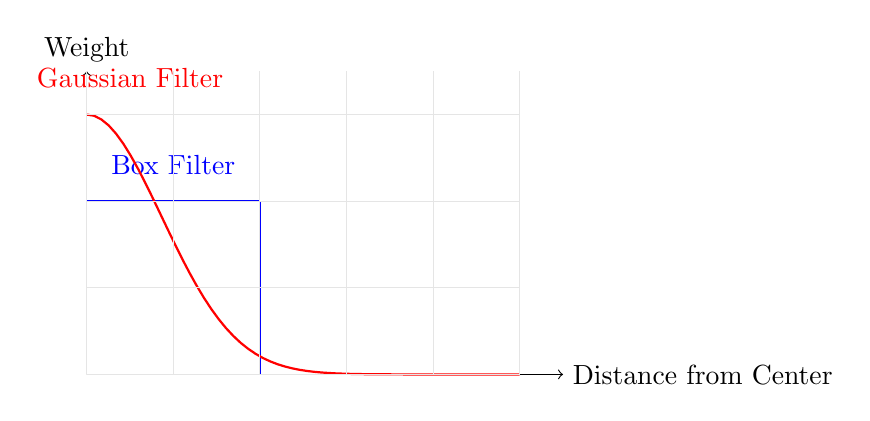
\begin{tikzpicture}[scale=1.1]
    % Axes
    \draw[->] (0,0) -- (5.5,0) node[right] {Distance from Center};
    \draw[->] (0,0) -- (0,3.5) node[above] {Weight};

    % Box filter (constant)
    \draw[thick,blue,domain=0:2,samples=2] plot (\x,2);
    \draw[thick,blue] (2,2) -- (2,0);
    \node[above,blue] at (1,2.2) {Box Filter};

    % Gaussian filter (bell curve)
    \draw[thick,red,domain=0:5,samples=60] plot (\x,{3*exp(-(\x-0)^2/1.5)});
    \node[above,red] at (0.5,3.2) {Gaussian Filter};

    % Grid
    \draw[step=1,gray!20] (0,0) grid (5,3.5);
\end{tikzpicture}
\end{center}

\textit{The Gaussian filter applies exponentially decreasing weights from the center, while the box filter uses uniform weights.}

\subsection*{Guideline for Selecting Gaussian Filter Kernel Size}
When selecting the kernel size for Gaussian filters, a common guideline is to use:
\[
\text{Kernel Size} = \lceil 6 \sigma \rceil
\]
For example, if we have \(\sigma = 7\):
\[
6 \times 7 = 42
\]
In this case, we would choose a kernel size of 43 to maintain an odd preference. However, it is important to note that there is no benefit in using a kernel size greater than \(\lceil 6 \sigma \rceil\).

\subsection*{Types of Padding}
\begin{center}
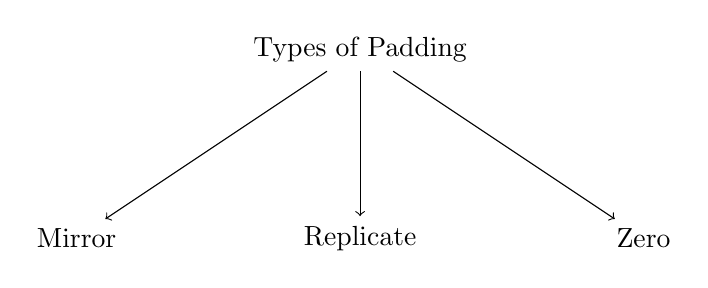
\begin{tikzpicture}[scale=1.2]
    % Root node
    \node (root) at (0,0) {Types of Padding};

    % Child nodes
    \node (mirror) at (-3,-2) {Mirror};
    \node (replicate) at (0,-2) {Replicate};
    \node (zero) at (3,-2) {Zero};

    % Arrows
    \draw[->] (root) -- (mirror);
    \draw[->] (root) -- (replicate);
    \draw[->] (root) -- (zero);
\end{tikzpicture}
\end{center}
\subsection*{Median Filter Example}

The median filter is a non-linear filter used to reduce noise in an image while preserving edges. It works by replacing each pixel value with the median value of the pixels in its neighborhood.

For a $3 \times 3$ matrix with the following values:

\[
\begin{bmatrix}
4 & 100 & 150 \\
25 & 78 & 16 \\
4 & 3 & 160
\end{bmatrix}
\]

To apply the median filter, we consider the values in the $3 \times 3$ neighborhood of each pixel. For the center pixel (78), the neighborhood values are:

\[
\{4, 100, 150, 25, 78, 16, 4, 3, 160\}
\]

Sorting these values gives:

\[
\{3, 4, 4, 16, 25, 78, 100, 150, 160\}
\]

The median value is the middle value in the sorted list, which is 25. Therefore, the center pixel (78) is replaced with 25.

This process is repeated for each pixel in the image, resulting in a new filtered image that reduces noise while maintaining important features.

\newpage
\section*{Sharpening Filters}

Sharpening filters are used to enhance edges and fine details in an image by amplifying high-frequency components. Unlike smoothing filters that blur an image, sharpening filters make transitions between pixel values more pronounced.

\subsection*{Blurring vs. Sharpening: Integration and Differentiation}

There is a fundamental mathematical relationship between blurring and sharpening operations:

\begin{itemize}
    \item \textbf{Blurring} corresponds to \textbf{integration}. Smoothing filters average neighboring pixel values, which is analogous to integrating a signal. This operation reduces high-frequency components and creates a smoother, more averaged representation of the image.
    
    \item \textbf{Sharpening} corresponds to \textbf{differentiation}. Sharpening filters compute differences between neighboring pixel values, which is analogous to differentiating a signal. This operation emphasizes edges and rapid intensity changes, enhancing high-frequency components.
\end{itemize}

This relationship reflects the inverse nature of these operations:
\[
\text{Integration} \leftrightarrow \text{Blurring (Low-pass filtering)}
\]
\[
\text{Differentiation} \leftrightarrow \text{Sharpening (High-pass filtering)}
\]

In practical terms, blurring smooths transitions by computing weighted averages, while sharpening highlights transitions by computing local derivatives or differences. Both operations are essential in image processing for different analytical and enhancement purposes.

\subsection*{First Order Derivatives}

First-order derivatives are used to detect edges in images by computing the rate of change of pixel intensity. The most common first-order derivative operators are the Sobel and Prewitt operators.

\subsubsection*{Sobel Operator}

The Sobel operator computes the gradient (first derivative) in both horizontal and vertical directions using two $3 \times 3$ kernels:

\textbf{Horizontal Sobel Kernel (} $S_x$ \textbf{):}
\[
S_x = \begin{bmatrix}
-1 & 0 & 1 \\
-2 & 0 & 2 \\
-1 & 0 & 1
\end{bmatrix}
\]

\textbf{Vertical Sobel Kernel (} $S_y$ \textbf{):}
\[
S_y = \begin{bmatrix}
-1 & -2 & -1 \\
0 & 0 & 0 \\
1 & 2 & 1
\end{bmatrix}
\]

The gradient magnitude is computed as:
\[
G = \sqrt{S_x^2 + S_y^2}
\]

\subsubsection*{Example Calculation}

Consider the following $3 \times 3$ image patch:

\[
f = \begin{bmatrix}
10 & 20 & 30 \\
15 & 25 & 35 \\
20 & 30 & 40
\end{bmatrix}
\]

\textbf{Applying} $S_x$ \textbf{(Horizontal Gradient):}
\[
S_x \text{ result} = (-1)(10) + (0)(20) + (1)(30) + (-2)(15) + (0)(25) + (2)(35) + (-1)(20) + (0)(30) + (1)(40)
\]
\[
= -10 + 0 + 30 - 30 + 0 + 70 - 20 + 0 + 40 = 80
\]

\textbf{Applying} $S_y$ \textbf{(Vertical Gradient):}
\[
S_y \text{ result} = (-1)(10) + (-2)(20) + (-1)(30) + (0)(15) + (0)(25) + (0)(35) + (1)(20) + (2)(30) + (1)(40)
\]
\[
= -10 - 40 - 30 + 0 + 0 + 0 + 20 + 60 + 40 = 40
\]

\textbf{Gradient Magnitude:}
\[
G = \sqrt{80^2 + 40^2} = \sqrt{6400 + 1600} = \sqrt{8000} \approx 89.44
\]

The gradient magnitude indicates the strength of the edge at this location. Higher values represent stronger edges.

\subsection*{Second Order Derivatives: Laplacian}

The Laplacian operator is a second-order derivative operator used for edge detection and image enhancement. It computes the sum of the second derivatives in both $x$ and $y$ directions and is particularly effective at detecting rapid intensity changes and edges.

\subsubsection*{Laplacian Definition}

The Laplacian operator is defined as:
\[
\nabla^2 f = \frac{\partial^2 f}{\partial x^2} + \frac{\partial^2 f}{\partial y^2}
\]

\subsubsection*{Laplacian Kernels}

The Laplacian can be approximated using discrete $3 \times 3$ kernels. The most common forms are:

\textbf{Standard Laplacian Kernel:}
\[
L = \begin{bmatrix}
0 & 1 & 0 \\
1 & -4 & 1 \\
0 & 1 & 0
\end{bmatrix}
\]
\[
\nabla^2 f(x,y)=f(x+1,y)+f(x-1,y)+f(x,y+1)+f(x,y-1)-4\,f(x,y)
\]
\textbf{Extended Laplacian Kernel (including diagonals):}
\[
L = \begin{bmatrix}
1 & 1 & 1 \\
1 & -8 & 1 \\
1 & 1 & 1
\end{bmatrix}
\]

\subsubsection*{Example Calculation}

Consider the following $3 \times 3$ image patch:

\[
f = \begin{bmatrix}
10 & 20 & 30 \\
15 & 25 & 35 \\
20 & 30 & 40
\end{bmatrix}
\]


\textbf{Applying the Standard Laplacian Kernel:}
\[
L \text{ result} = (0)(10) + (1)(20) + (0)(30) + (1)(15) + (-4)(25) + (1)(35) + (0)(20) + (1)(30) + (0)(40)
\]
\[
= 0 + 20 + 0 + 15 - 100 + 35 + 0 + 30 + 0 = 0
\]

\subsubsection*{Properties of the Laplacian}

\begin{itemize}
    \item \textbf{Isotropic:} The Laplacian is rotation-invariant, meaning it responds equally to edges in all directions.
    \item \textbf{Edge Detection:} Produces zero values in uniform regions and non-zero values at edges.
    \item \textbf{Sensitive to Noise:} Being a second-order derivative, the Laplacian is more sensitive to noise than first-order operators.
    \item \textbf{Zero Crossing:} Edges are often located at zero-crossings of the Laplacian (transitions from positive to negative or vice versa).
    \item \textbf{Double Edges:} Can produce double edges around actual edge locations due to the second derivative nature.
\end{itemize}

\subsubsection*{Comparison: First Order vs. Second Order}

\begin{center}
\begin{tabular}{|c|c|c|}
\hline
\textbf{Property} & \textbf{First Order (Sobel)} & \textbf{Second Order (Laplacian)} \\
\hline
Derivative Type & First derivative (gradient) & Second derivative \\
\hline
Edge Detection & Detects edge location and direction & Detects edge transitions (zero-crossings) \\
\hline
Noise Sensitivity & Less sensitive & More sensitive \\
\hline
Computational Cost & Moderate & Low \\
\hline
Output Type & Gradient magnitude and direction & Scalar value (zero-crossing) \\
\hline
\end{tabular}
\end{center}

\subsection*{Roberts Operator}

The Roberts operator is another first-order derivative operator used for edge detection. It uses two $2 \times 2$ kernels to compute gradients in diagonal directions.

\textbf{Roberts Kernel 1 (Diagonal):}
\[
R_1 = \begin{bmatrix}
1 & 0 \\
0 & -1
\end{bmatrix}
\]

\textbf{Roberts Kernel 2 (Anti-Diagonal):}
\[
R_2 = \begin{bmatrix}
0 & 1 \\
-1 & 0
\end{bmatrix}
\]

The gradient magnitude is computed as:
\[
G = \sqrt{R_1^2 + R_2^2}
\]

\subsubsection*{Comparison: Sobel vs. Roberts}

\begin{center}
\begin{tabular}{|c|c|c|}
\hline
\textbf{Property} & \textbf{Sobel} & \textbf{Roberts} \\
\hline
Kernel Size & $3 \times 3$ & $2 \times 2$ \\
\hline
Computational Cost & Moderate & Low \\
\hline
Edge Detection & Strong edges & Thin, precise edges \\
\hline
Noise Sensitivity & Moderate & Higher \\
\hline
Smoothing Effect & Slight (averaging) & None \\
\hline
\end{tabular}
\end{center}
\newpage
\subsection*{Unsharp Masking and Highboost Filtering}

Unsharp masking and highboost filtering are sharpening techniques that enhance edges and fine details by combining the original image with a blurred (unsharp) version of itself.

\subsubsection*{Unsharp Masking}

Unsharp masking works by subtracting a blurred version of the image from the original image to create a high-pass filtered result. This technique is based on the principle that edges and fine details are preserved in the original image but removed in the blurred version.
\\ \\
\textbf{Formula:}
\[
g(x,y) = f(x,y) - \text{blur}[f(x,y)]
\] where $\text{blur}[f(x,y)]$ is the blurred version of the image.
\\ \\
Alternatively, the result can be added back to the original to create a sharpened image:
\[
g(x,y) = f(x,y) + k \cdot [f(x,y) - \text{blur}[f(x,y)]]
\] where $k$ is a scaling factor controlling the amount of sharpening.
$k > 1$ results in highboost filtering while $k = 1$ results in standard unsharp masking.

\newpage
\section*{Summary Table of Image Enhancement Techniques}
\begin{center}
\begin{tabular}{|L{2.5cm}|L{3.5cm}|L{5cm}|L{3.5cm}|}
\hline
\textbf{Domain} & \textbf{Technique} & \textbf{Primary Goal / Effect} & \textbf{Key Mechanism} \\
\hline
\multicolumn{4}{|l|}{\textbf{Intensity Transformations (Point Operations)}} \\
\hline
Intensity (Point Ops) & Image Negative & Reverses colors to enhance \textbf{dark area details}. & $s = (L-1) - r$ \\
\hline
Intensity (Point Ops) & Log Transformation & \textbf{Expands dark pixels}, compresses light pixels. & Uses a logarithmic function. \\
\hline
Intensity (Point Ops) & Power-Law ($\gamma$ Transform) & Controls overall brightness/contrast based on $\gamma$ value. & $s = cr^{\gamma}$ \\
\hline
Intensity (Point Ops) & Contrast Stretching & Expands the intensity range to use the \textbf{full scale}. & Piecewise linear function. \\
\hline
\multicolumn{4}{|l|}{\textbf{Histogram Processing}} \\
\hline
Histogram Processing & Histogram Equalization (Global) & Enhances image contrast by aiming for a \textbf{uniform histogram}. & Discrete Cumulative Distribution Function (CDF). \\
\hline
Histogram Processing & Histogram Matching (Specification) & Changes the image's histogram to match a \textbf{specific desired shape}. & Equating two equalized variables. \\
\hline
Histogram Processing & Local Histogram Processing & Enhances \textbf{details over small areas}. & Applied globally within a moving local neighborhood. \\
\hline
\multicolumn{4}{|l|}{\textbf{Spatial Filtering (Neighborhood Operations)}} \\
\hline
Smoothing (Lowpass Filters) & Box Filter (Averaging) & \textbf{Blurs} the image to reduce noise. & Replaces pixel value with the average of its neighbors. \\
\hline
Smoothing (Lowpass Filters) & Median Filter & Excellent reduction of \textbf{salt-and-pepper noise}. & Replaces pixel value with the \textbf{median} of its neighbors. \\
\hline
Sharpening (Highpass Filters) & Laplacian (2nd Derivative) & Enhances \textbf{fine detail} and sharp transitions. & Uses second derivative convolution kernel. \\
\hline
Sharpening (Highpass Filters) & Gradient (Roberts/Sobel) & Highlights \textbf{prominent edges}. & Uses first derivative kernels (vector magnitude). \\
\hline
Sharpening (Highpass Filters) & Unsharp Masking / Highboost & Sharpens image details. & $\text{Sharpened} = \text{Original} + k(\text{Original} - \text{Blurred})$. \\
\hline
\end{tabular}
\end{center}


\newpage
\begin{center}
\begin{tabular}{|L{4cm}|L{4cm}|L{7.5cm}|}
\hline
\textbf{Image Condition/Problem} & \textbf{Recommended Techniques} & \textbf{Primary Goal \& Mechanism} \\
\hline
\multicolumn{3}{|l|}{\textbf{Contrast and Intensity Adjustment}} \\
\hline
\textbf{Overall Low Contrast} (Clustered histogram) & \textbf{Global Histogram Equalization} & Enhances **overall contrast** by forcing the histogram towards a uniform distribution. \\
\hline
\textbf{Low Contrast + Washed-out/Light Image} & \textbf{Contrast Stretching} & Expands the intensity range to span the **ideal full intensity range** using piecewise linear transformation. \\
\hline
\textbf{Low Contrast with Specific Brightness Need} & \textbf{Histogram Matching (Specification)} & Transforms the histogram to match a **specific desired shape** by equating two equalized transformation variables. \\
\hline
\textbf{Very Dark Image} (Loss of shadow detail) & \textbf{Log Transformation} or \textbf{Power-Law ($\gamma < 1$)} & **Expands dark pixels** using a non-linear curve that rises steeply at low input values. \\
\hline
\textbf{White/Gray Details Embedded in Dark Background} & \textbf{Image Negatives} & **Reverses** the intensity levels using the linear inversion formula: $g(x,y) = (L-1) - f(x,y)$. \\
\hline
\textbf{Fine Details Hidden in Dark Areas} (Local problem) & \textbf{Local Histogram Processing} & Enhances **details over small areas** by applying histogram methods within a moving neighborhood. \\
\hline
\multicolumn{3}{|l|}{\textbf{Noise Reduction, Smoothing, and Sharpening}} \\
\hline
\textbf{General Noise Reduction} (Smoothing) & \textbf{Box Filter} or \textbf{Gaussian Filter} & Reduces **sharp transitions in intensity** (noise) using linear spatial filtering (convolution). \\
\hline
\textbf{Salt-and-Pepper Noise} (Impulse Noise) & \textbf{Median Filter} (Non-linear) & Achieves very good **noise reduction** by replacing the center pixel with the **median** of its neighborhood. \\
\hline
\textbf{Image is Too Smooth/Blurry} (Needs Detail Recovery) & \textbf{Sharpening Filters} & Highlights intensity transitions (edges) by computing the **digital differentiation**. \\
\hline
\textbf{Enhancing Fine Detail} (Texture) & \textbf{Laplacian} (Second Derivative) & Enhances **fine detail much better** than the first derivative by adding the calculated Laplacian image to the original. \\
\hline
\textbf{Enhancing Prominent Edges} (Object Outlines) & \textbf{Gradient} (First Derivative, e.g., Sobel) & Provides a **stronger response to significant intensity transitions** using first-order derivative operators. \\
\hline
\textbf{Controlled Sharpening/Edge Boost} & \textbf{Unsharp Masking} or \textbf{Highboost Filtering} & Sharpens image details using the difference formula: $\text{Sharpened} = \text{Original} + k(\text{Original} - \text{Blurred})$ with $k \geq 1$. \\
\hline
\end{tabular}
\end{center}

\newpage
\section*{Fourier Series Analysis on Images}

The Fourier transform is a fundamental tool in image processing that converts an image from the spatial domain to the frequency domain. This transformation enables analysis and manipulation of image frequencies, which is essential for filtering, compression, and feature extraction.

\subsection*{Spatial Domain vs. Frequency Domain}

\begin{center}
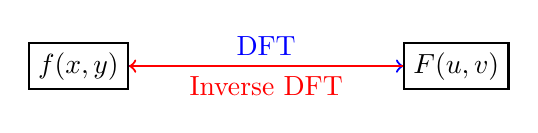
\begin{tikzpicture}[scale=1.2]
    % Spatial domain
    \node[rectangle,draw,thick] (spatial) at (0,0) {$f(x,y)$};
    
    % Frequency domain
    \node[rectangle,draw,thick] (freq) at (4,0) {$F(u,v)$};
    
    % Top arrow (DFT)
    \draw[->,thick,blue] (spatial) -- (freq) node[midway,above] {DFT};
    
    % Bottom arrow (Inverse DFT)
    \draw[<-,thick,red] (spatial) -- (freq) node[midway,below] {Inverse DFT};
\end{tikzpicture}
\end{center}

The Discrete Fourier Transform (DFT) converts spatial domain information into frequency domain representation, revealing the frequency components that compose the image. The Inverse DFT reverses this process to recover the spatial domain image.

\subsection*{Steps for Frequency Domain Filtering}

The following procedure describes the complete process of converting an image from the spatial domain to the frequency domain, applying filtering, and converting back:

\begin{enumerate}
    \item \textbf{Pad the Input Image:} Given an input image $f(x,y)$ of size $M \times N$, pad the image to size $P \times Q$, where:
    \[
    P = 2M, \quad Q = 2N
    \]
    This zero-padding prevents circular convolution artifacts and improves computational efficiency.
    
    \item \textbf{Multiply by Phase Factor:} Multiply the padded image by $(-1)^{x+y}$ to centre the DFT of $f(x,y)$:
    \[
    f_{\text{padded}}(x,y) \cdot (-1)^{x+y}
    \]
    This shifts the zero-frequency component to the center of the frequency domain.
    
    \item \textbf{Compute the DFT:} Calculate the Discrete Fourier Transform to obtain $F(u,v)$:
    \[
    F(u,v) = \sum_{x=0}^{P-1} \sum_{y=0}^{Q-1} f_{\text{padded}}(x,y) \cdot e^{-j2\pi(ux/P + vy/Q)}
    \]
    
    \item \textbf{Construct Filter Transfer Function:} Create a real, symmetric filter transfer function $H(u,v)$ of size $P \times Q$ with centre at $(P/2, Q/2)$. The filter design depends on the desired frequency response (lowpass, highpass, bandpass, etc.).
    
    \item \textbf{Apply Filter in Frequency Domain:} Form the product $G(u,v)$ by multiplying the filter and DFT elementwise:
    \[
    G(u,v) = H(u,v) \cdot F(u,v)
    \]
    
    \item \textbf{Compute Inverse DFT:} Calculate the Inverse Discrete Fourier Transform and multiply by $(-1)^{x+y}$ to shift the zero-frequency component back:
    \[
    g_{\text{filtered}}(x,y) = \text{IDFT}[G(u,v)] \cdot (-1)^{x+y}
    \]
    
    \item \textbf{Extract Result:} The final filtered image is obtained by extracting the $M \times N$ region from the top left quadrant of $g_{\text{filtered}}(x,y)$.
\end{enumerate}

\subsubsection*{Key Considerations}

\begin{itemize}
    \item \textbf{Zero-Padding:} Padding prevents aliasing and circular convolution effects that would occur without padding.
    \item \textbf{Phase Centering:} The $(-1)^{x+y}$ multiplication ensures that the zero-frequency (DC) component is at the center of the frequency domain, making visualization and filter design more intuitive.
    \item \textbf{Filter Design:} The transfer function $H(u,v)$ is customized based on the filtering objective (noise reduction, edge enhancement, etc.).
    \item \textbf{Computational Efficiency:} Using FFT (Fast Fourier Transform) significantly reduces computation time compared to direct DFT calculation.
\end{itemize}


\subsection*{Summary: Centering, DFT, and the 4x4 Example}

Here is the complete summary of our journey, tying together the conceptual tricks, the specific Mathematica settings, and the raw math using your concrete $4 \times 4$ example.

\subsubsection*{1. The Concept: Why We Center the Data}

\textbf{The Problem:} By default, the standard DFT places the zero-frequency (DC) term---which represents the total energy/brightness of the image---at the origin $(0,0)$ (top-left corner). This splits the "low frequency" details across the four corners, making it impossible to apply a simple circular filter in the middle.

\textbf{The Fix:} Multiply the input image by a checkerboard pattern $(-1)^{x+y}$.

\textbf{The Effect:} This modulation uses the "Shift Property" of the Fourier Transform, shifting the frequency spectrum by half the image size ($M/2, N/2$), moving the DC spike from the corner to the geometric center.

\subsubsection*{2. The Concrete Example (Non-Uniform $4 \times 4$ Matrix)}

We used this $4 \times 4$ matrix to illustrate the process:
\[
A = 
\begin{bmatrix}
1 & 2 & 9 & 7 \\
99 & 88 & 66 & 22 \\
55 & 1000 & 999 & 9998 \\
44 & 22 & 5555 & 199
\end{bmatrix}
\]

\textbf{The Summation Expansion (How We Got 18,166):}

The DC component (all exponents become 1):
\[
F(0,0) = \sum_{x=1}^{4} \sum_{y=1}^{4} A_{x,y}
\]
Row sums:
\begin{align*}
\text{Row 1:} &\quad 1 + 2 + 9 + 7 = 19 \\
\text{Row 2:} &\quad 99 + 88 + 66 + 22 = 275 \\
\text{Row 3:} &\quad 55 + 1000 + 999 + 9998 = 12052 \\
\text{Row 4:} &\quad 44 + 22 + 5555 + 199 = 5820 \\
\end{align*}
Total sum: $19 + 275 + 12052 + 5820 = \mathbf{18,166}$.

\textbf{Resulting Matrices:}

\emph{Uncentered DFT (Standard):} Energy at $(0,0)$.
\[
\begin{bmatrix}
\mathbf{18166} & 11153 & 4510 & 11153 \\
13249 & 14553 & 11279 & 3644 \\
5976 & 9977 & 15376 & 9977 \\
13249 & 3644 & 11279 & 14553
\end{bmatrix}
\]

\emph{Centered DFT (After Trick):} Energy at center $(2,2)$.
\[
\begin{bmatrix}
15376 & 9977 & 5976 & 9977 \\
11279 & 14553 & 13249 & 3644 \\
4510 & 11153 & \mathbf{18166} & 11153 \\
11279 & 3644 & 13249 & 14553
\end{bmatrix}
\]

\subsubsection*{3. The Parameters: \texttt{FourierParameters -> \{1, -1\}}}

\begin{itemize}
    \item $a = 1$ (Amplitude): Scaling factor is $1/n^{(1-1)/2} = 1$, so the result is the raw sum (not divided by 16).
    \item $b = -1$ (Phase): Exponent is $-2\pi i$, the standard forward transform.
\end{itemize}

\subsubsection*{4. The Final Equation}

\textbf{Input:} Use the centered image $B1$ where $B1_{x,y} = A_{x,y} \cdot (-1)^{x+y}$.

\textbf{Base Formula:} The unscaled DFT is $\sum \text{Data} \cdot e^{-2\pi i \dots}$.

\textbf{Indexing:} Mathematica counts from $1$ to $N$ (not $0$ to $N-1$), so subtract $1$ from every coordinate in the exponent.

\textbf{Final Equation:}
\[
BF_{u,v} = \sum_{x=1}^{M} \sum_{y=1}^{N} B1_{x,y} \, e^{-2\pi i \left( \frac{(u-1)(x-1)}{M} + \frac{(v-1)(y-1)}{N} \right)}
\]
This equation takes every pixel from your centered image $B1$, compares it against a wave frequency defined by $(u,v)$, sums up the results, and stores it in the output spectrum $BF$.

\subsubsection*{Mathematica Implementation Example (Lecture 4.2--4.5)}

Below is a step-by-step Mathematica implementation for frequency domain filtering (ideal low pass filter), including spectrum centering, zero-padding, filtering, and reconstruction:

\begin{verbatim}
(* Load and convert image to grayscale byte matrix *)
i = Import["ExampleData/lena.tif"];
A = ImageData[i, "Byte"];
{Md, Nd} = Dimensions[A];

(* Center the spectrum *)
CM = Table[(-1)^(i + j), {i, 1, Md}, {j, 1, Nd}];
B = A * CM;

(* Zero-pad to double size *)
B1 = ArrayPad[B, {{0, Md}, {0, Nd}}];
{P, Q} = Dimensions[B1];

(* Compute the centered Fourier transform *)
BF = Fourier[B1, FourierParameters -> {1, -1}];

(* Construct ideal low pass filter *)
dis[u_, v_] := Sqrt[(u - Md)^2 + (v - Nd)^2];
D0 = 20;
H = Table[If[dis[u, v] <= D0, 1, 0], {u, 1, P}, {v, 1, Q}];

(* Apply filter in frequency domain *)
G = BF * H;

(* Inverse Fourier transform and take real part *)
R = Re[InverseFourier[G, FourierParameters -> {1, -1}]];

(* Extract top-left quadrant *)
R1 = Take[R, {1, Md}, {1, Nd}];

(* Reverse centering *)
R2 = R1 * CM;

(* Display result *)
Image[R2, "Byte"]
\end{verbatim}
This code demonstrates the full process: centering, padding, filtering, and reconstructing the filtered image in Mathematica.

\newpage


\newpage
\section*{Low Pass Filters}

Low pass filters are used to remove high-frequency components from an image while preserving low-frequency information. This results in image smoothing and noise reduction. In the frequency domain, low pass filters attenuate frequencies above a cutoff frequency while allowing lower frequencies to pass through.

\subsection*{Ideal Low Pass Filter}

The ideal low pass filter is the simplest type of frequency domain filter. It completely removes all frequency components beyond a specified cutoff distance $D_0$ from the origin in the frequency domain.

\subsubsection*{Transfer Function}

The transfer function for an ideal low pass filter is defined as:

\[
H(u,v) = \begin{cases}
1, & \text{if } D(u,v) \leq D_0 \\
0, & \text{if } D(u,v) > D_0
\end{cases}
\]

where $D(u,v) = \sqrt{(u - P/2)^2 + (v - Q/2)^2}$ is the distance from the center of the frequency domain, and $D_0$ is the cutoff distance.

\subsubsection*{Characteristics}

\begin{itemize}
    \item \textbf{Sharp Cutoff:} The ideal filter has a sharp transition at the cutoff frequency $D_0$.
    \item \textbf{Ringing Artifacts:} Due to the sharp frequency cutoff, ideal low pass filters produce ringing artifacts (also called Gibbs phenomenon) at edges in the filtered image.
    \item \textbf{Simple Implementation:} Easy to implement and understand.
    \item \textbf{Not Practical:} Rarely used in practice due to the ringing artifacts it introduces.
\end{itemize}

\subsubsection*{Visualization}

\begin{center}
\begin{tikzpicture}[scale=1.1]
    % Axes
    \draw[->] (0,0) -- (5.5,0) node[right] {Distance from Center $D(u,v)$};
    \draw[->] (0,0) -- (0,3.2) node[above] {$H(u,v)$};

    % Ideal filter response
    \draw[thick,blue] (0,2.5) -- (2.5,2.5);
    \draw[thick,blue] (2.5,2.5) -- (2.5,0);
    \draw[thick,blue] (2.5,0) -- (5,0);

    % Cutoff line
    \draw[dashed,red] (2.5,0) -- (2.5,2.5);
    \node[below,red] at (2.5,0) {$D_0$};

    % Labels
    \node[left] at (0,2.5) {1};
    \node[above right,blue] at (3.5,0.5) {Ideal Low Pass Filter};
\end{tikzpicture}
\end{center}


\subsection*{Gaussian Low Pass Filter}

The Gaussian low pass filter provides a smooth transition between frequencies that are passed and frequencies that are attenuated. It avoids the sharp cutoff of the ideal filter, resulting in significantly fewer ringing artifacts.

\subsubsection*{Transfer Function}

The transfer function for a Gaussian low pass filter is defined as:

\[
H(u,v) = e^{-D(u,v)^2 / (2\sigma^2)}
\]

where $\sigma$ controls the spread of the Gaussian function. Alternatively, using cutoff frequency $D_0$:

\[
H(u,v) = e^{-D(u,v)^2 / (2D_0^2)}
\]

\subsubsection*{Characteristics}

\begin{itemize}
    \item \textbf{Smooth Transition:} Provides a gradual transition from pass-band to stop-band.
    \item \textbf{No Ringing:} Eliminates the ringing artifacts associated with ideal filters.
    \item \textbf{Natural Smoothing:} Produces more natural-looking smoothed images.
    \item \textbf{Commonly Used:} Widely used in practical applications due to its smooth frequency response.
\end{itemize}

\subsubsection*{Visualization}

\begin{center}
\begin{tikzpicture}[scale=1.1]
    % Axes
    \draw[->] (0,0) -- (5.5,0) node[right] {Distance from Center $D(u,v)$};
    \draw[->] (0,0) -- (0,3.2) node[above] {$H(u,v)$};

    % Gaussian filter response
    \draw[thick,blue,domain=0:5,samples=80] plot (\x,{2.5*exp(-(\x)^2/1.5)});

    % Cutoff reference
    \draw[dashed,red] (2.5,0) -- (2.5,{2.5*exp(-2.5^2/1.5)});
    \node[below,red] at (2.5,0) {$D_0$};

    % Labels
    \node[left] at (0,2.5) {1};
    \node[above right,blue] at (3.5,1.5) {Gaussian Low Pass Filter};
\end{tikzpicture}
\end{center}

\subsection*{Butterworth Low Pass Filter}

The Butterworth low pass filter provides a compromise between the ideal and Gaussian filters. It has a tunable parameter $n$ (order) that controls the sharpness of the cutoff, allowing adjustment between smoothness and transition sharpness.

\subsubsection*{Transfer Function}

The transfer function for a Butterworth low pass filter of order $n$ is defined as:

\[
H(u,v) = \frac{1}{1 + \left[\frac{D(u,v)}{D_0}\right]^{2n}}
\]

where:
\begin{itemize}
    \item $D_0$ is the cutoff frequency (distance at which $H = 0.5$).
    \item $n$ is the order of the filter, controlling the sharpness of the cutoff.
\end{itemize}

\subsubsection*{Characteristics}

\begin{itemize}
    \item \textbf{Adjustable Sharpness:} Order $n$ controls the transition sharpness:
    \begin{itemize}
        \item $n = 1$: Smooth, similar to Gaussian.
        \item $n = 2, 3, \ldots$: Progressively sharper cutoff.
        \item $n \to \infty$: Approaches ideal filter behavior.
    \end{itemize}
    \item \textbf{Minimal Ringing:} Much less ringing than ideal filter but sharper than Gaussian.
    \item \textbf{Versatile:} Provides flexibility to balance between smoothness and cutoff sharpness.
    \item \textbf{Maximally Flat:} In the pass-band, the frequency response is maximally flat (no ripple).
\end{itemize}

\subsubsection*{Visualization}

\begin{center}
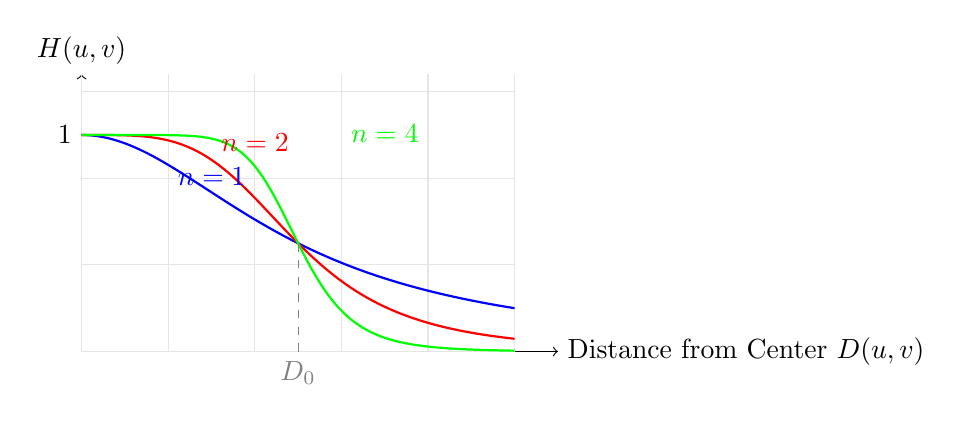
\begin{tikzpicture}[scale=1.1]
    % Axes
    \draw[->] (0,0) -- (5.5,0) node[right] {Distance from Center $D(u,v)$};
    \draw[->] (0,0) -- (0,3.2) node[above] {$H(u,v)$};

    % Grid
    \draw[step=1,gray!20] (0,0) grid (5,3.2);

    % Butterworth curves for different orders
    \draw[thick,blue,domain=0:5,samples=80] plot (\x,{2.5/(1+(\x/2.5)^2)});
    \draw[thick,red,domain=0:5,samples=80] plot (\x,{2.5/(1+(\x/2.5)^4)});
    \draw[thick,green,domain=0:5,samples=80] plot (\x,{2.5/(1+(\x/2.5)^8)});

    % Cutoff reference
    \draw[dashed,gray] (2.5,0) -- (2.5,1.25);
    \node[below,gray] at (2.5,0) {$D_0$};

    % Labels
    \node[left] at (0,2.5) {1};
    \node[above right,blue] at (1,1.8) {$n=1$};
    \node[above right,red] at (1.5,2.2) {$n=2$};
    \node[above right,green] at (3,2.3) {$n=4$};
\end{tikzpicture}
\end{center}

\subsubsection*{Mathematica Implementation}

\begin{verbatim}
(* Butterworth Low Pass Filter Example *)
BLPF[img_,D0_,order_]:=Module[{A, Md, Nd, CM, B, B1,P,Q,
BF,filterButterworth,filteredDFT,inverseDFT,phaseShift,filteredShifted,resultImg },
A=ImageData[ColorConvert[img,"Grayscale"],"Byte"];{Md,Nd}=Dimensions[A];
CM=Table[(-1)^(i+j),{i,1,Md},{j,1,Nd}];B=A*CM;
B1=ArrayPad[B,{{0,Md},{0,Nd}}];{P,Q}=Dimensions[B1];
BF=Fourier[B1,FourierParameters->{1,-1}];
filterButterworth=Table[1/(1+(Sqrt[(u-P/2)^2+(v-Q/2)^2]/D0)^(2*order)),{u,0,P-1},{v,0,Q-1}];
filteredDFT=BF*filterButterworth;
inverseDFT=InverseFourier[filteredDFT,FourierParameters->{1, -1}];
phaseShift=Table[(-1)^(x+y),{x,0,P-1},{y,0,Q-1}];
filteredShifted=inverseDFT*phaseShift;
resultImg=Take[Re[filteredShifted],{1,Md},{1,Nd}];
Image[resultImg,"Byte"]
]

i = Import["https://boofcv.org/images/thumb/6/66/Kodim17_noisy.jpg/300px-Kodim17_noisy.jpg"]

Manipulate[BLPF[i,cutoff,order],{cutoff,1,255,1},{order,1,4}]
\end{verbatim}

\subsubsection*{Comparison: Low Pass Filters}

\begin{center}
\begin{tabular}{|c|c|c|c|}
\hline
\textbf{Property} & \textbf{Ideal} & \textbf{Gaussian} & \textbf{Butterworth} \\
\hline
Cutoff Sharpness & Very sharp & Smooth & Adjustable (via $n$) \\
\hline
Ringing Artifacts & Severe & None & Minimal \\
\hline
Transition Smoothness & Abrupt & Gradual & Tunable \\
\hline
Practical Use & Rare & Very common & Common \\
\hline
Parameter Control & $D_0$ only & $D_0$ only & $D_0$ and $n$ \\
\hline
Computational Cost & Low & Low & Low \\
\hline
Best For & Theoretical analysis & General smoothing & Balanced applications \\
\hline
\end{tabular}
\end{center}

\newpage
\section*{High Pass Filters}

High pass filters are used to enhance high-frequency components in an image while attenuating low-frequency information. This results in edge enhancement and detail sharpening. In the frequency domain, high pass filters attenuate frequencies below a cutoff frequency while allowing higher frequencies to pass through.

\subsection*{Ideal High Pass Filter}

The ideal high pass filter is the complementary operation to the ideal low pass filter. It completely removes all frequency components within a specified cutoff distance $D_0$ from the origin while preserving all components beyond this distance.

\subsubsection*{Transfer Function}

The transfer function for an ideal high pass filter is defined as:

\[
H(u,v) = \begin{cases}
0, & \text{if } D(u,v) \leq D_0 \\
1, & \text{if } D(u,v) > D_0
\end{cases}
\]

where $D(u,v) = \sqrt{(u - P/2)^2 + (v - Q/2)^2}$ is the distance from the center of the frequency domain, and $D_0$ is the cutoff distance.

\subsubsection*{Characteristics}

\begin{itemize}
    \item \textbf{Sharp Cutoff:} The ideal filter has a sharp transition at the cutoff frequency $D_0$.
    \item \textbf{Ringing Artifacts:} Due to the sharp frequency cutoff, ideal high pass filters produce ringing artifacts at edges in the filtered image.
    \item \textbf{Edge Enhancement:} Emphasizes edges and fine details while suppressing smooth regions.
    \item \textbf{Not Practical:} Rarely used in practice due to the ringing artifacts it introduces.
\end{itemize}

\subsubsection*{Visualization}

\begin{center}
\begin{tikzpicture}[scale=1.1]
    % Axes
    \draw[->] (0,0) -- (5.5,0) node[right] {Distance from Center $D(u,v)$};
    \draw[->] (0,0) -- (0,3.2) node[above] {$H(u,v)$};

    % Ideal high pass filter response
    \draw[thick,blue] (0,0) -- (2.5,0);
    \draw[thick,blue] (2.5,0) -- (2.5,2.5);
    \draw[thick,blue] (2.5,2.5) -- (5,2.5);

    % Cutoff line
    \draw[dashed,red] (2.5,0) -- (2.5,2.5);
    \node[below,red] at (2.5,0) {$D_0$};

    % Labels
    \node[left] at (0,2.5) {1};
    \node[above right,blue] at (3.5,2.5) {Ideal High Pass Filter};
\end{tikzpicture}
\end{center}

\subsection*{Gaussian High Pass Filter}

The Gaussian high pass filter provides a smooth transition between frequencies that are attenuated and frequencies that are passed. It avoids the sharp cutoff of the ideal filter, resulting in significantly fewer ringing artifacts.

\subsubsection*{Transfer Function}

The transfer function for a Gaussian high pass filter is defined as:

\[
H(u,v) = 1 - e^{-D(u,v)^2 / (2\sigma^2)}
\]

where $\sigma$ controls the spread of the Gaussian function. Alternatively, using cutoff frequency $D_0$:

\[
H(u,v) = 1 - e^{-D(u,v)^2 / (2D_0^2)}
\]

\subsubsection*{Characteristics}

\begin{itemize}
    \item \textbf{Smooth Transition:} Provides a gradual transition from stop-band to pass-band.
    \item \textbf{No Ringing:} Eliminates the ringing artifacts associated with ideal filters.
    \item \textbf{Natural Sharpening:} Produces more natural-looking sharpened images.
    \item \textbf{Commonly Used:} Widely used in practical edge detection and sharpening applications.
\end{itemize}

\subsubsection*{Visualization}

\begin{center}
\begin{tikzpicture}[scale=1.1]
    % Axes
    \draw[->] (0,0) -- (5.5,0) node[right] {Distance from Center $D(u,v)$};
    \draw[->] (0,0) -- (0,3.2) node[above] {$H(u,v)$};

    % Gaussian high pass filter response
    \draw[thick,blue,domain=0:5,samples=80] plot (\x,{2.5*(1-exp(-(\x)^2/1.5))});

    % Cutoff reference
    \draw[dashed,red] (2.5,0) -- (2.5,{2.5*(1-exp(-2.5^2/1.5))});
    \node[below,red] at (2.5,0) {$D_0$};

    % Labels
    \node[left] at (0,2.5) {1};
    \node[above right,blue] at (3.5,2) {Gaussian High Pass Filter};
\end{tikzpicture}
\end{center}


\subsection*{Butterworth High Pass Filter}

The Butterworth high pass filter provides a compromise between the ideal and Gaussian filters. It has a tunable parameter $n$ (order) that controls the sharpness of the cutoff, allowing adjustment between smoothness and transition sharpness.

\subsubsection*{Transfer Function}

The transfer function for a Butterworth high pass filter of order $n$ is defined as:

\[
H(u,v) = \frac{1}{1 + \left[\frac{D_0}{D(u,v)}\right]^{2n}}
\]

where:
\begin{itemize}
    \item $D_0$ is the cutoff frequency (distance at which $H = 0.5$).
    \item $n$ is the order of the filter, controlling the sharpness of the cutoff.
    \item $D(u,v)$ is the distance from the center of the frequency domain.
\end{itemize}

\subsubsection*{Characteristics}

\begin{itemize}
    \item \textbf{Adjustable Sharpness:} Order $n$ controls the transition sharpness:
    \begin{itemize}
        \item $n = 1$: Smooth, similar to Gaussian.
        \item $n = 2, 3, \ldots$: Progressively sharper cutoff.
        \item $n \to \infty$: Approaches ideal filter behavior.
    \end{itemize}
    \item \textbf{Minimal Ringing:} Much less ringing than ideal filter but sharper than Gaussian.
    \item \textbf{Versatile:} Provides flexibility to balance between smoothness and cutoff sharpness.
    \item \textbf{Maximally Flat:} In the pass-band, the frequency response is maximally flat (no ripple).
\end{itemize}

\subsubsection*{Visualization}

\begin{center}
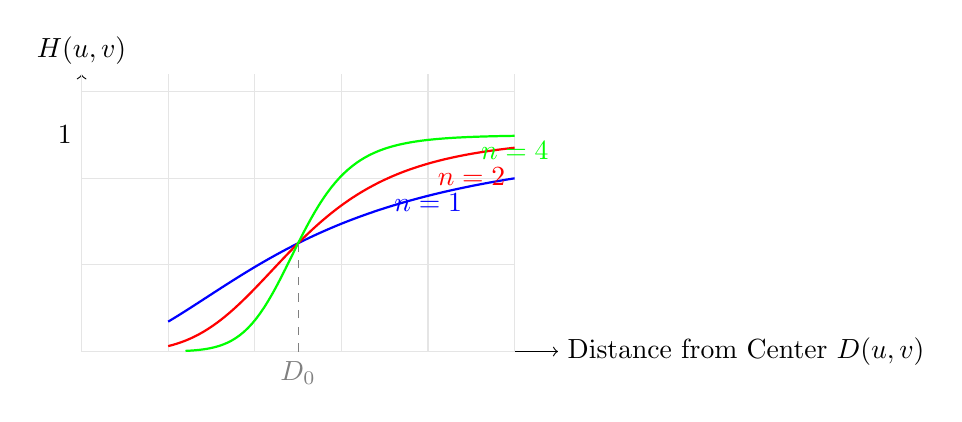
\begin{tikzpicture}[scale=1.1]
    % Axes
    \draw[->] (0,0) -- (5.5,0) node[right] {Distance from Center $D(u,v)$};
    \draw[->] (0,0) -- (0,3.2) node[above] {$H(u,v)$};

    % Grid
    \draw[step=1,gray!20] (0,0) grid (5,3.2);

    % Butterworth curves for different orders
    \draw[thick,blue,domain=1:5,samples=80] plot (\x,{2.5/(1+(2.5/\x)^2)});
    \draw[thick,red,domain=1:5,samples=80] plot (\x,{2.5/(1+(2.5/\x)^4)});
    \draw[thick,green,domain=1.2:5,samples=80] plot (\x,{2.5/(1+(2.5/\x)^8)});

    % Cutoff reference
    \draw[dashed,gray] (2.5,0) -- (2.5,1.25);
    \node[below,gray] at (2.5,0) {$D_0$};

    % Labels
    \node[left] at (0,2.5) {1};
    \node[above right,blue] at (3.5,1.5) {$n=1$};
    \node[above right,red] at (4,1.8) {$n=2$};
    \node[above right,green] at (4.5,2.1) {$n=4$};
\end{tikzpicture}
\end{center}

\subsubsection*{Mathematica Implementation}

\begin{verbatim}BHPF[img_, D0_, order_] := 

 Module[{A, Md, Nd, CM, B, B1, P, Q, BF, filterButterworth, 
    filteredDFT, inverseDFT, phaseShift, filteredShifted, resultImg}, 

  A = ImageData[ColorConvert[img, "Grayscale"], "Byte"]; {Md, Nd} = Dimensions[A];

  CM = Table[(-1)^(i + j), {i, 1, Md}, {j, 1, Nd}]; B = A*CM;
  B1 = ArrayPad[B, {{0, Md}, {0, Nd}}]; {P, Q} = Dimensions[B1];
  BF = Fourier[B1, FourierParameters -> {1, -1}];
  filterButterworth = 
   Table[1/(1 + (D0/(Sqrt[(u - P/2)^2 + (v - Q/2)^2] + 0.0001))^(2*
          order)), {u, 0, P - 1}, {v, 0, Q - 1}]; 
  filteredDFT = BF*filterButterworth;
  inverseDFT = 
   InverseFourier[filteredDFT, FourierParameters -> {1, -1}];
  phaseShift = Table[(-1)^(x + y), {x, 0, P - 1}, {y, 0, Q - 1}];
  filteredShifted = inverseDFT*phaseShift;
  resultImg = Take[Re[filteredShifted], {1, Md}, {1, Nd}];
  Image[resultImg, "Byte"]]

i = Import["https://boofcv.org/images/thumb/6/66/Kodim17_noisy.jpg/300px-Kodim17_noisy.jpg"]
Manipulate[BHPF[i, cutoff, order], {cutoff, 1, 255, 1}, {order, 1, 4}]
\end{verbatim}

\subsubsection*{Comparison: High Pass Filters}

\begin{center}
\begin{tabular}{|c|c|c|c|}
\hline
\textbf{Property} & \textbf{Ideal} & \textbf{Gaussian} & \textbf{Butterworth} \\
\hline
Cutoff Sharpness & Very sharp & Smooth & Adjustable (via $n$) \\
\hline
Ringing Artifacts & Severe & None & Minimal \\
\hline
Transition Smoothness & Abrupt & Gradual & Tunable \\
\hline
Practical Use & Rare & Very common & Common \\
\hline
Parameter Control & $D_0$ only & $D_0$ only & $D_0$ and $n$ \\
\hline
Computational Cost & Low & Low & Low \\
\hline
Best For & Theoretical analysis & General sharpening & Balanced applications \\
\hline
\end{tabular}
\end{center}

\subsection*{Comparison: Low Pass vs. High Pass Filters}

\begin{center}
\begin{tabular}{|c|c|c|}
\hline
\textbf{Property} & \textbf{Low Pass Filter} & \textbf{High Pass Filter} \\
\hline
Primary Effect & Smoothing, blur reduction & Sharpening, edge enhancement \\
\hline
Frequency Response & Attenuates high frequencies & Attenuates low frequencies \\
\hline
Removes & Noise, fine details & Smooth regions, DC component \\
\hline
Preserves & Large-scale structure & Edges and fine details \\
\hline
Transfer Function & $H(u,v) = 1$ for $D \leq D_0$ & $H(u,v) = 1$ for $D > D_0$ \\
\hline
Application & Noise reduction preprocessing & Edge detection, feature enhancement \\
\hline
Output Appearance & Blurred, smoothed image & Enhanced edges, high contrast \\
\hline
\end{tabular}
\end{center}

\section*{Laplacian in Frequency Domain}

The Laplacian operator can be implemented in the frequency domain as an alternative to spatial domain convolution. This approach is particularly useful when working with large images or when combining multiple frequency domain operations.

\subsection*{Laplacian Transfer Function}

In the frequency domain, the Laplacian operator is represented by its transfer function:

\[
H(u,v) = -4\pi^2(u^2 + v^2)
\]

However, for practical implementation and to avoid amplifying noise excessively, a normalized version is often used:

\[
H(u,v) = -(u^2 + v^2)
\]

or equivalently:

\[
H(u,v) = -D(u,v)^2 = -[(u - P/2)^2 + (v - Q/2)^2]
\]

\subsection*{Properties}

\begin{itemize}
    \item \textbf{High-Pass Nature:} The Laplacian is a high-pass filter that enhances high-frequency components (edges and details).
    \item \textbf{Zero at DC:} The transfer function is zero at the origin (DC component), eliminating the average intensity from the output.
    \item \textbf{Isotropic:} Responds equally to edges in all directions.
    \item \textbf{Noise Amplification:} Amplifies high-frequency noise, so preprocessing with smoothing is often recommended.
\end{itemize}

\subsection*{Frequency Domain Laplacian Implementation}

The procedure for applying the Laplacian in the frequency domain follows the standard 7-step frequency domain filtering approach:

\begin{enumerate}
    \item Pad the input image to size $P \times Q$ where $P = 2M$ and $Q = 2N$.
    \item Multiply by $(-1)^{x+y}$ to center the DFT.
    \item Compute the DFT of the padded image.
    \item Construct the Laplacian transfer function $H(u,v) = -(u - P/2)^2 - (v - Q/2)^2$.
    \item Apply the filter: $G(u,v) = H(u,v) \cdot F(u,v)$.
    \item Compute the inverse DFT and multiply by $(-1)^{x+y}$.
    \item Extract the $M \times N$ result from the top-left quadrant.
\end{enumerate}

\subsection*{Mathematica Implementation}

\begin{verbatim}
(* Laplacian Filter in Frequency Domain *)
(* Step 1: Load and Pad Image *)
img = ExampleData[{"TestImage", "Lena"}];
{M, N} = ImageDimensions[img];
P = 2*M; Q = 2*N;
imgData = ImageData[img, "Real"];
paddedImg = PadRight[imgData, {P, Q}, 0];

(* Step 2: Phase Shift *)
phaseShift = Table[(-1)^(x + y), {x, 0, P-1}, {y, 0, Q-1}];
shiftedImg = paddedImg * phaseShift;

(* Step 3: Compute DFT *)
dftResult = Fourier[shiftedImg];

(* Step 4: Construct Laplacian Transfer Function *)
filterLaplacian = Table[
    -((u - P/2)^2 + (v - Q/2)^2),
    {u, 0, P-1}, {v, 0, Q-1}
];

(* Step 5: Apply Filter *)
filteredDFT = dftResult * filterLaplacian;

(* Step 6: Inverse DFT *)
inverseDFT = InverseFourier[filteredDFT];
filteredShifted = inverseDFT * phaseShift;

(* Step 7: Extract Result *)
resultImg = Take[Re[filteredShifted], {1, M}, {1, N}];
resultLaplacian = Image[Rescale[resultImg, {Min[resultImg], Max[resultImg]}, 
                                                          {0, 1}]];

(* Display *)
Row[{Image[imgData], resultLaplacian}, Spacer[10]]
\end{verbatim}

\subsection*{Comparison: Spatial vs. Frequency Domain Laplacian}

\begin{center}
\begin{tabular}{|c|c|c|}
\hline
\textbf{Aspect} & \textbf{Spatial Domain} & \textbf{Frequency Domain} \\
\hline
Implementation & Direct convolution with kernel & FFT-based multiplication \\
\hline
Computational Efficiency & Slower for large images & Faster for large images (FFT) \\
\hline
Kernel Size & Fixed $3 \times 3$ & Flexible (full image size) \\
\hline
Boundary Handling & Requires padding strategy & Automatic (circular) \\
\hline
Intuitive Understanding & Immediate (local differences) & Requires frequency interpretation \\
\hline
Combination with Other Filters & Difficult & Easy (multiply transfer functions) \\
\hline
Noise Sensitivity & Moderate & High (amplifies all frequencies) \\
\hline
\end{tabular}
\end{center}

\newpage
\section*{Unsharp Masking, Highboost Filtering, and High Frequency Emphasis Filtering (Mathematica Example)}

\begin{verbatim}
UnsharpMaskG[im_, D0_, k1_, k2_] := (
    img = ColorConvert[im, "Grayscale"];
    A = ImageData[img, "Byte"];
    d = Dimensions[A];
    M1 = d[[1]]; (* number of rows *)
    M2 = d[[2]]; (* number of columns *)
    CMat = Array[1 - 2 Mod[#1 + #2, 2] &, {M1, M2}];
    B = A*CMat;
    B1 = ArrayPad[B, {{0, M1 + 1}, {0, M2 + 1}}];
    d = Dimensions[B1];
    P = d[[1]];
    Q = d[[2]];
    BF = Fourier[B1, FourierParameters -> {1, -1}];
    H2 = GaussianMatrix[{{M1, M2}, D0}, Standardized -> False];
    H2n = H2/H2[[M1 + 1, M2 + 1]];
    H = 1 - H2n;
    G = BF*(k1 + k2*H);
    R = Re[InverseFourier[G, FourierParameters -> {1, -1}]];
    R1 = Take[R, {1, M1}, {1, M2}];
    R1 = R1*CMat;
    Grid[{{"Original image", "Filtered image", 
         "Filtered image after intensity transformation"}, {im, 
         Image[R1, "Byte"], HistogramTransform[Image[R1, "Byte"]]}}, 
     Spacings -> {2, 2, 2}, Frame -> All]
)
UnsharpMaskG[i4, 70, 0.5, 0.75]
\end{verbatim}




\subsection*{Explanation: Unsharp Masking, Highboost Filtering, and High Frequency Emphasis Filtering}

\textbf{Unsharp masking} is a classic image sharpening technique. It works by subtracting a blurred (lowpass filtered) version of the image from the original, emphasizing edges and fine details (high frequencies). The result can be added back to the original image for enhanced sharpness.

\textbf{Highboost filtering} generalizes unsharp masking by scaling the high-frequency component before adding it back. The formula is:
\[
g(x, y) = f(x, y) + k \cdot [f(x, y) - \text{blur}(f(x, y))]
\]
where $k > 1$ produces stronger sharpening.

\textbf{High frequency emphasis filtering} is a further generalization, where both the original and the high-frequency component are scaled independently:
\[
G(u, v) = [k_1 + k_2 \cdot H_{HPF}(u, v)] \cdot F(u, v)
\]
where $H_{HPF}$ is a highpass filter (e.g., Gaussian), $k_1$ controls the original image, and $k_2$ controls the high-frequency emphasis.

\textbf{In the code above:}
- The image is converted to grayscale and centered for frequency domain processing.
- A Gaussian highpass filter is constructed.
- The filter is applied in the frequency domain with weights $k_1$ and $k_2$ (high frequency emphasis).
- The result is inverse transformed, de-centered, and displayed.
- The third column shows the result after histogram equalization for better contrast.

This approach allows flexible sharpening, from subtle (unsharp masking) to aggressive (highboost), and can emphasize high-frequency details as needed.

\subsection*{How to Choose $k_1$ and $k_2$ in High Frequency Emphasis Filtering}

The parameters $k_1$ and $k_2$ in high frequency emphasis filtering control the contribution of the original image and the high-frequency (sharpened) component, respectively:
\[
G(u, v) = [k_1 + k_2 \cdot H_{HPF}(u, v)] \cdot F(u, v)
\]
where $H_{HPF}(u, v)$ is the highpass filter transfer function.

\begin{itemize}
    \item \textbf{$k_1$ (Low Frequency Weight):} Controls the amount of the original (low-frequency) image retained. Typical values are $0 \leq k_1 \leq 1$. Setting $k_1 = 1$ keeps the original image fully; $k_1 < 1$ reduces its contribution.
    \item \textbf{$k_2$ (High Frequency Weight):} Controls the strength of the high-frequency emphasis (sharpening). Typical values are $0 < k_2 \leq 1$. Increasing $k_2$ increases sharpening, but too large a value can amplify noise and cause artifacts.
\end{itemize}

\newpage

\section*{Mathematica Code Examples for Frequency Domain Filtering}
\subsection*{Calculating the Fourier Series: Small $4 \times 4$ Example}

Below is Mathematica code to compute the 2D Discrete Fourier Transform (DFT) for your $4 \times 4$ matrix example, both uncentered and centered (using the $(-1)^{x+y}$ trick):

\begin{verbatim}
(* Define the 4x4 matrix *)
A = {{1, 2, 9, 7},
    {99, 88, 66, 22},
    {55, 1000, 999, 9998},
    {44, 22, 5555, 199}};

(* Uncentered DFT *)
DFTuncentered = Fourier[A, FourierParameters -> {1, -1}];

(* Centered DFT: multiply by (-1)^(x+y) *)
CM = Table[(-1)^(i + j), {i, 1, 4}, {j, 1, 4}];
Acentered = A * CM;
DFTcentered = Fourier[Acentered, FourierParameters -> {1, -1}];

(* Display magnitude spectra *)
Grid[{
  {"Original Matrix", "Uncentered DFT (Magnitude)", "Centered DFT (Magnitude)"},
  {MatrixForm[A], MatrixForm[Abs[DFTuncentered]], MatrixForm[Abs[DFTcentered]]}
}]
\end{verbatim}

This code shows how to compute the DFT for your matrix, both with and without centering, and displays the magnitude spectra for comparison.

\subsection*{Ideal Low Pass Filter (ILPF)}
\begin{verbatim}
ILPF[im_, D0_] := (
    img = ColorConvert[im, "Grayscale"];
    A = ImageData[img, "Byte"];
    {M1, M2} = Dimensions[A];
    CMat = Table[(-1)^(i + j), {i, 1, M1}, {j, 1, M2}];
    B = A * CMat; (* Centering the image *)
    B1 = ArrayPad[B, {{0, M1}, {0, M2}}];
    {P, Q} = Dimensions[B1];
    BF = Fourier[B1, FourierParameters -> {1, -1}];
    dis[u_, v_] := Sqrt[(u - M1)^2 + (v - M2)^2];
    H = Table[If[dis[u, v] <= D0, 1, 0], {u, 1, P}, {v, 1, Q}];
    G = BF * H;
    R = Re[InverseFourier[G, FourierParameters -> {1, -1}]];
    R1 = Take[R, {1, M1}, {1, M2}];
    R1 = R1 * CMat;
    Grid[{{"Original image", "Filter", 
    "Filtered image before de-centering, still with padding", "Filtered image"},
        {img, Image[H], Image[R, "Byte"], Image[R1, "Byte"]}}, 
        Spacings -> {2, 2, 2, 2}, Frame -> All]
)
\end{verbatim}

\newpage
\subsection*{Ideal High Pass Filter (IHPF)}
\begin{verbatim}
IHPF[im_, D0_] := (
    img = ColorConvert[im, "Grayscale"];
    A = ImageData[img, "Byte"];
    {M1, M2} = Dimensions[A];
    CMat = Table[(-1)^(i + j), {i, 1, M1}, {j, 1, M2}];
    B = A * CMat;
    B1 = ArrayPad[B, {{0, M1}, {0, M2}}];
    {P, Q} = Dimensions[B1];
    BF = Fourier[B1, FourierParameters -> {1, -1}];
    dis[u_, v_] := Sqrt[(u - M1)^2 + (v - M2)^2];
    H = Table[If[dis[u, v] <= D0, 1, 0], {u, 1, P}, {v, 1, Q}];
    G = BF * (1 - H);
    R = Re[InverseFourier[G, FourierParameters -> {1, -1}]];
    R1 = Take[R, {1, M1}, {1, M2}];
    R1 = R1 * CMat;
    Grid[{{"Original image", "Filter", 
    "Filtered image before de-centering, still with padding", "Filtered image"},
        {img, Image[H], Image[R, "Byte"], 
        Image[R1, "Byte"]}}, Spacings -> {2, 2, 2, 2}, Frame -> All]
)
\end{verbatim}

\subsection*{Gaussian Low Pass Filter (GLPF)}
\begin{verbatim}
GLPFfast[im_, D0_] := (
    img = ColorConvert[im, "Grayscale"];
    A = ImageData[img, "Byte"];
    d = Dimensions[A];
    M1 = d[[1]];
    M2 = d[[2]];
    CMat = Array[1 - 2 Mod[#1 + #2, 2] &, {M1, M2}];
    B = A * CMat;
    B1 = ArrayPad[B, {{0, M1 + 1}, {0, M2 + 1}}];
    d = Dimensions[B1];
    P = d[[1]];
    Q = d[[2]];
    BF = Fourier[B1, FourierParameters -> {1, -1}];
    H2 = GaussianMatrix[{{M1, M2}, D0}, Standardized -> False];
    H2n = H2 / H2[[M1 + 1, M2 + 1]];
    G = BF * H2n;
    R = Re[InverseFourier[G, FourierParameters -> {1, -1}]];
    R1 = Take[R, {1, M1}, {1, M2}];
    R1 = R1 * CMat;
    Grid[{{"Original image", "Filter", 
    "Filtered image before de-centering, still with padding", "Filtered image"},
        {img, Image[H2n], Image[R, "Byte"], Image[R1, "Byte"]}}, 
        Spacings -> {2, 2, 2, 2}, Frame -> All]
)
\end{verbatim}

\newpage
\subsection*{Gaussian High Pass Filter (GHPF)}
\begin{verbatim}
GHPFfast[im_, D0_] := (
    img = ColorConvert[im, "Grayscale"];
    A = ImageData[img, "Byte"];
    d = Dimensions[A];
    M1 = d[[1]];
    M2 = d[[2]];
    CMat = Array[1 - 2 Mod[#1 + #2, 2] &, {M1, M2}];
    B = A * CMat;
    B1 = ArrayPad[B, {{0, M1 + 1}, {0, M2 + 1}}];
    d = Dimensions[B1];
    P = d[[1]];
    Q = d[[2]];
    BF = Fourier[B1, FourierParameters -> {1, -1}];
    H2 = GaussianMatrix[{{M1, M2}, D0}, Standardized -> False];
    H2n = H2 / H2[[M1 + 1, M2 + 1]];
    G = BF * (1 - H2n);
    R = Re[InverseFourier[G, FourierParameters -> {1, -1}]];
    R1 = Take[R, {1, M1}, {1, M2}];
    R1 = R1 * CMat;
    Grid[{{"Original image", "Filter", 
    "Filtered image before de-centering, still with padding", "Filtered image"},
        {img, Image[1 - H2n], Image[R, "Byte"], Image[R1, "Byte"]}}, 
        Spacings -> {2, 2, 2, 2}, Frame -> All]
)
\end{verbatim}

\subsection*{Unsharp Masking with Gaussian High Pass Filter}
\begin{verbatim}
UnsharpMaskG[im_, D0_, k1_, k2_] := (
    img = ColorConvert[im, "Grayscale"];
    A = ImageData[img, "Byte"];
    d = Dimensions[A];
    M1 = d[[1]];
    M2 = d[[2]];
    CMat = Array[1 - 2 Mod[#1 + #2, 2] &, {M1, M2}];
    B = A * CMat;
    B1 = ArrayPad[B, {{0, M1 + 1}, {0, M2 + 1}}];
    d = Dimensions[B1];
    P = d[[1]];
    Q = d[[2]];
    BF = Fourier[B1, FourierParameters -> {1, -1}];
    H2 = GaussianMatrix[{{M1, M2}, D0}, Standardized -> False];
    H2n = H2 / H2[[M1 + 1, M2 + 1]];
    H = 1 - H2n;
    G = BF * (k1 + k2 * H);
    R = Re[InverseFourier[G, FourierParameters -> {1, -1}]];
    R1 = Take[R, {1, M1}, {1, M2}];
    R1 = R1 * CMat;
    Grid[{{"Original image", "Filtered image", "Filtered image after intensity transformation"},
        {im, Image[R1, "Byte"], HistogramTransform[Image[R1, "Byte"]]}}, 
        Spacings -> {2, 2, 2}, Frame -> All]
)
\end{verbatim}

\subsection*{Comparison: Spatial vs. Frequency Domain Unsharp Masking}

\begin{center}
\begin{tabular}{|c|c|c|}
\hline
\textbf{Aspect} & \textbf{Spatial Domain} & \textbf{Frequency Domain} \\
\hline
Implementation & Explicit blur + subtraction & Single transfer function \\
\hline
Computational Efficiency & Slower (multiple convolutions) & Faster (single FFT) \\
\hline
Filter Flexibility & Limited to kernel size & Flexible frequency control \\
\hline
Control & Direct visual parameters & Frequency-based parameters \\
\hline
Combination & Difficult (sequential ops) & Easy (multiply functions) \\
\hline
Intuitive Understanding & High (visual process) & Lower (frequency interpretation) \\
\hline
\end{tabular}
\end{center}
\vspace{4pt}

\section*{Band Reject, Band Pass, and Notch Filters}

This section provides Mathematica code for frequency domain band reject, band pass, and notch filters. Each filter is illustrated with a schematic graph showing its frequency response, followed by the corresponding Mathematica implementation.

\subsection*{Mathematica Code Examples}

\textbf{1. Ideal Band Reject Filter}
\begin{verbatim}
IdealBandRejectFilter[img_, D0_, W_] := Module[
    {data, rows, cols, P, Q, paddedData, centeredData, 
    F, H, d, G, gInverse, gReal, finalData, result},
    data = ImageData[ColorConvert[img, "Grayscale"]];
    {rows, cols} = Dimensions[data];
    P = 2*rows; Q = 2*cols;
    paddedData = ArrayPad[data, {{0, rows}, {0, cols}}];
    centeredData = Table[paddedData[[x, y]]*(-1)^(x + y), {x, 1, P}, 
    {y, 1, Q}];
    F = Fourier[centeredData, FourierParameters -> {1, -1}];
    H = Table[
        d = Sqrt[(u - P/2)^2 + (v - Q/2)^2];
        If[D0 - W/2 <= d <= D0 + W/2, 0, 1],
        {u, 1, P}, {v, 1, Q}
    ];
    G = F*H;
    gInverse = InverseFourier[G, FourierParameters -> {1, -1}];
    gReal = Re[gInverse];
    finalData = Table[gReal[[x, y]]*(-1)^(x + y), {x, 1, P}, {y, 1, Q}];
    result = Take[finalData, {1, rows}, {1, cols}];
    Image[result]
]
\end{verbatim}

\textbf{2. Gaussian Band Reject Filter}
\begin{verbatim}
GaussianBandRejectFilter[img_, D0_, W_] := Module[
    {data, rows, cols, P, Q, paddedData, centeredData, 
    F, H, d, G, gInverse, gReal, finalData, result},
    data = ImageData[ColorConvert[img, "Grayscale"]];
    {rows, cols} = Dimensions[data];
    P = 2*rows; Q = 2*cols;
    paddedData = ArrayPad[data, {{0, rows}, {0, cols}}];
    centeredData = Table[paddedData[[x, y]]*(-1)^(x + y), {x, 1, P}, 
    {y, 1, Q}];
    F = Fourier[centeredData, FourierParameters -> {1, -1}];
    H = Table[
        d = Sqrt[(u - P/2)^2 + (v - Q/2)^2];
        If[d == 0, 1, 1 - Exp[-0.5*((d^2 - D0^2)/(d*W))^2]],
        {u, 1, P}, {v, 1, Q}
    ];
    G = F*H;
    gInverse = InverseFourier[G, FourierParameters -> {1, -1}];
    gReal = Re[gInverse];
    finalData = Table[gReal[[x, y]]*(-1)^(x + y), {x, 1, P}, {y, 1, Q}];
    result = Take[finalData, {1, rows}, {1, cols}];
    Image[result]
]
\end{verbatim}

\textbf{3. Butterworth Band Reject Filter}
\begin{verbatim}
ButterworthBandRejectFilter[img_, D0_, W_, n_] := Module[
    {data, rows, cols, P, Q, paddedData, centeredData, 
    F, H, d, denom, G, gInverse, gReal, finalData, result},
    data = ImageData[ColorConvert[img, "Grayscale"]];
    {rows, cols} = Dimensions[data];
    P = 2*rows; Q = 2*cols;
    paddedData = ArrayPad[data, {{0, rows}, {0, cols}}];
    centeredData = Table[paddedData[[x, y]]*(-1)^(x + y), 
    {x, 1, P}, {y, 1, Q}];
    F = Fourier[centeredData, FourierParameters -> {1, -1}];
    H = Table[
        d = Sqrt[(u - P/2)^2 + (v - Q/2)^2];
        denom = (d^2 - D0^2) + 0.00001;
        1/(1 + ((d*W)/denom)^(2*n)),
        {u, 1, P}, {v, 1, Q}
    ];
    G = F*H;
    gInverse = InverseFourier[G, FourierParameters -> {1, -1}];
    gReal = Re[gInverse];
    finalData = Table[gReal[[x, y]]*(-1)^(x + y), {x, 1, P}, {y, 1, Q}];
    result = Take[finalData, {1, rows}, {1, cols}];
    Image[result]
]
\end{verbatim}

\textbf{4. Ideal Band Pass Filter}
\begin{verbatim}
IdealBandPassFilter[img_, D0_, W_] := Module[
    {data, rows, cols, P, Q, paddedData, centeredData, 
    F, H, d, G, gInverse, gReal, finalData, result},
    data = ImageData[ColorConvert[img, "Grayscale"]];
    {rows, cols} = Dimensions[data];
    P = 2*rows; Q = 2*cols;
    paddedData = ArrayPad[data, {{0, rows}, {0, cols}}];
    centeredData = Table[paddedData[[x, y]]*(-1)^(x + y), 
    {x, 1, P}, {y, 1, Q}];
    F = Fourier[centeredData, FourierParameters -> {1, -1}];
    H = Table[
        d = Sqrt[(u - P/2)^2 + (v - Q/2)^2];
        If[D0 - W/2 <= d <= D0 + W/2, 1, 0],
        {u, 1, P}, {v, 1, Q}
    ];
    G = F*H;
    gInverse = InverseFourier[G, FourierParameters -> {1, -1}];
    gReal = Re[gInverse];
    finalData = Table[gReal[[x, y]]*(-1)^(x + y), {x, 1, P}, 
    {y, 1, Q}];
    result = Take[finalData, {1, rows}, {1, cols}];
    Image[result]
]
\end{verbatim}

\textbf{5. Gaussian Band Pass Filter}
\begin{verbatim}
GaussianBandPassFilter[img_, D0_, W_] := Module[
    {data, rows, cols, P, Q, paddedData, centeredData, 
    F, H, d, G, gInverse, gReal, finalData, result},
    data = ImageData[ColorConvert[img, "Grayscale"]];
    {rows, cols} = Dimensions[data];
    P = 2*rows; Q = 2*cols;
    paddedData = ArrayPad[data, {{0, rows}, {0, cols}}];
    centeredData = Table[paddedData[[x, y]]*(-1)^(x + y), {x, 1, P}, 
    {y, 1, Q}];
    F = Fourier[centeredData, FourierParameters -> {1, -1}];
    H = Table[
        d = Sqrt[(u - P/2)^2 + (v - Q/2)^2];
        If[d == 0, 0, Exp[-0.5*((d^2 - D0^2)/(d*W))^2]],
        {u, 1, P}, {v, 1, Q}
    ];
    G = F*H;
    gInverse = InverseFourier[G, FourierParameters -> {1, -1}];
    gReal = Re[gInverse];
    finalData = Table[gReal[[x, y]]*(-1)^(x + y), {x, 1, P}, {y, 1, Q}];
    result = Take[finalData, {1, rows}, {1, cols}];
    Image[result]
]
\end{verbatim}

\textbf{6. Butterworth Band Pass Filter}
\begin{verbatim}
ButterworthBandPassFilter[img_, D0_, W_, n_] := Module[
    {data, rows, cols, P, Q, paddedData, centeredData, 
    F, H, d, denom, G, gInverse, gReal, finalData, result},
    data = ImageData[ColorConvert[img, "Grayscale"]];
    {rows, cols} = Dimensions[data];
    P = 2*rows; Q = 2*cols;
    paddedData = ArrayPad[data, {{0, rows}, {0, cols}}];
    centeredData = Table[paddedData[[x, y]]*(-1)^(x + y), 
    {x, 1, P}, {y, 1, Q}];
    F = Fourier[centeredData, FourierParameters -> {1, -1}];
    H = Table[
        d = Sqrt[(u - P/2)^2 + (v - Q/2)^2];
        denom = (d^2 - D0^2) + 0.00001;
        1 - 1/(1 + ((d*W)/denom)^(2*n)),
        {u, 1, P}, {v, 1, Q}
    ];
    G = F*H;
    gInverse = InverseFourier[G, FourierParameters -> {1, -1}];
    gReal = Re[gInverse];
    finalData = Table[gReal[[x, y]]*(-1)^(x + y), {x, 1, P}, {y, 1, Q}];
    result = Take[finalData, {1, rows}, {1, cols}];
    Image[result]
]
\end{verbatim}

\textbf{7. Butterworth Notch Filter}
\begin{verbatim}
ButterworthNotchFilter[img_, centers_, D0_, n_] := Module[
    {data, rows, cols, P, Q, paddedData, centeredData, 
    F, H, d1, d2, G, gInverse, gReal, finalData, result},
    data = ImageData[ColorConvert[img, "Grayscale"]];
    {rows, cols} = Dimensions[data];
    P = 2*rows; Q = 2*cols;
    paddedData = ArrayPad[data, {{0, rows}, {0, cols}}];
    centeredData = Table[paddedData[[x, y]]*(-1)^(x + y), {x, 1, P}, 
    {y, 1, Q}];
    F = Fourier[centeredData, FourierParameters -> {1, -1}];
    H = Table[
        Product[
            d1 = Sqrt[(u - P/2 - c[[1]])^2 + (v - Q/2 - c[[2]])^2];
            d2 = Sqrt[(u - P/2 + c[[1]])^2 + (v - Q/2 + c[[2]])^2];
            If[d1*d2 == 0, 0, 1/(1 + (D0^2/(d1*d2))^n)],
            {c, centers}
        ],
        {u, 1, P}, {v, 1, Q}
    ];
    G = F*H;
    gInverse = InverseFourier[G, FourierParameters -> {1, -1}];
    gReal = Re[gInverse];
    finalData = Table[gReal[[x, y]]*(-1)^(x + y), {x, 1, P}, {y, 1, Q}];
    result = Take[finalData, {1, rows}, {1, cols}];
    Image[result]
]
\end{verbatim}

\textbf{Usage Example:}
\begin{verbatim}
img = Import["ExampleData/lena.tif"];
D0 = 60; W = 30; n = 2;
notchCenters = {{40, 40}, {40, -40}}; notchRadius = 10;

outIdealBR = IdealBandRejectFilter[img, D0, W];
outGaussBR = GaussianBandRejectFilter[img, D0, W];
outButterBR = ButterworthBandRejectFilter[img, D0, W, n];
outIdealBP = IdealBandPassFilter[img, D0, W];
outGaussBP = GaussianBandPassFilter[img, D0, W];
outButterBP = ButterworthBandPassFilter[img, D0, W, n];
outNotch = ButterworthNotchFilter[img, notchCenters, notchRadius, n];

(* Display results in a grid *)
LabelImg[image_, text_] := Column[{image, Style[text, 
FontFamily -> "Helvetica", 12, Gray]}, Center];
Grid[{
    {LabelImg[img, "Original Image"], 
    LabelImg[outNotch, "7. Notch Filter"]},
    {LabelImg[outIdealBR, "1. Ideal Band Reject"], 
    LabelImg[outGaussBR, "2. Gaussian Band Reject"]},
    {LabelImg[outButterBR, "3. Butterworth Band Reject"], SpanFromLeft},
    {LabelImg[outIdealBP, "4. Ideal Band Pass"], 
    LabelImg[outGaussBP, "5. Gaussian Band Pass"]},
    {LabelImg[outButterBP, "6. Butterworth Band Pass"], SpanFromLeft}
}, Frame -> All, Spacings -> {1, 1}, Alignment -> Center]
\end{verbatim}

\subsection*{Summary}

\begin{itemize}
    \item Notch filters are essential for removing periodic noise in images.
    \item The filter is constructed to target specific frequency locations.
    \item Butterworth and Gaussian notch filters are preferred for smooth transitions and minimal artifacts.
    \item The process involves identifying noise frequencies, constructing the filter, applying it in the frequency domain, and transforming back to the spatial domain.
\end{itemize}

\newpage

\section*{Quick Reference: Which Frequency Domain Filter to Use?}

\begin{center}
\begin{tabular}{|L{3.5cm}|L{4cm}|L{5cm}|L{3.5cm}|}
\hline
\textbf{Scenario / Problem} & \textbf{Recommended Filter} & \textbf{Effect / Rationale} & \textbf{Typical Parameters} \\
\hline
General smoothing, noise reduction & \textbf{Gaussian Low Pass} & Smooths image, minimal ringing, natural blur & $D_0 = 10$--$50$ (depends on image size) \\
\hline
Aggressive smoothing, theoretical study & \textbf{Ideal Low Pass} & Removes all frequencies above cutoff, but causes ringing & $D_0 = 10$--$50$ \\
\hline
Smoothing with adjustable sharpness & \textbf{Butterworth Low Pass} & Tunable transition, balance between ideal and Gaussian & $D_0 = 10$--$50$, $n = 2$--$4$ \\
\hline
Edge enhancement, detail sharpening & \textbf{Gaussian High Pass} & Enhances edges, smooth transition, minimal artifacts & $D_0 = 10$--$50$ \\
\hline
Strong edge enhancement, theoretical & \textbf{Ideal High Pass} & Sharp cutoff, strong edge emphasis, severe ringing & $D_0 = 10$--$50$ \\
\hline
Sharpening with tunable sharpness & \textbf{Butterworth High Pass} & Adjustable edge enhancement, less ringing than ideal & $D_0 = 10$--$50$, $n = 2$--$4$ \\
\hline
Controlled sharpening, edge boost & \textbf{Unsharp Masking / Highboost} & Adds scaled high-frequency detail, flexible control & $k_1 = 1$, $k_2 = 0.5$--$1$, $D_0 = 20$--$70$ \\
\hline
Fine detail enhancement & \textbf{Laplacian (Frequency Domain)} & Highlights rapid intensity changes, isotropic & No parameter (or scale $H(u,v)$ as needed) \\
\hline
Remove periodic noise (stripes, interference) & \textbf{Band Reject / Notch Filter} & Suppresses specific frequency bands or points & $D_0 =$ distance to noise, $W =$ width, $n = 2$--$4$ \\
\hline
Enhance features in a frequency range & \textbf{Band Pass Filter} & Keeps only desired frequency band & $D_0 =$ center, $W =$ width, $n = 2$--$4$ \\
\hline
\end{tabular}
\end{center}

\begin{itemize}
    \item \textbf{Low Pass:} Use for denoising and smoothing. Gaussian is safest for natural images.
    \item \textbf{High Pass:} Use for sharpening and edge enhancement. Gaussian or Butterworth preferred.
    \item \textbf{Band Reject/Notch:} Use to remove periodic or localized frequency noise.
    \item \textbf{Unsharp/Highboost:} Use for controlled sharpening with $k_2$ for strength.
    \item \textbf{Laplacian:} Use for isotropic edge enhancement.
    \item \textbf{Parameter choice:} $D_0$ should be $\sim$2--10\% of image diagonal for most images; $n=2$ is a good default for Butterworth.
\end{itemize}

\newpage
\section*{Color Image Processing}

This section demonstrates how to process color images in Mathematica, including color space conversion, channel separation, intensity transformations, color segmentation, and color balancing. Each example is accompanied by code and explanations.

\subsubsection*{1. Creating an RGB Image from a Matrix}

You can create a small color image by specifying a $2 \times 3$ matrix, where each entry is a list of three values (R, G, B) between 0 and 1.

\begin{verbatim}
(* Create a 2x3 RGB matrix with random values *)
m = RandomReal[{0, 1}, {2, 3, 3}];

(* Display as an RGB image *)
Image[m, ColorSpace -> "RGB"]

(* Display as an HSB image (interprets the numbers as HSB, not RGB) *)
Image[m, ColorSpace -> "HSB"]
\end{verbatim}

\textbf{Explanation:} The same matrix can be interpreted as RGB or HSB. The appearance will change because the numbers are interpreted differently in each color space.

\subsubsection*{2. Color Space Analysis and Conversion}

Given a color image (e.g., the "Mandrill" test image):

\begin{verbatim}
(* Load the image *)
img = ExampleData[{"TestImage", "Mandrill"}];

(* a. Find the color space *)
ImageColorSpace[img]  (* Output: "RGB" *)

(* b. Visualize the image as if its data were HSB *)
Image[img, ColorSpace -> "HSB"]

(* c. Convert the image to HSB properly *)
imgHSB = ColorConvert[img, "HSB"];
ImageColorSpace[imgHSB]  (* Output: "HSB" *)

(* d. Extract the underlying data matrices *)
A1 = ImageData[img];      (* RGB data *)
A2 = ImageData[imgHSB];   (* HSB data *)

A1[[1, 1]]  (* First pixel in RGB *)
A2[[1, 1]]  (* First pixel in HSB *)

(* e. Visualize the HSB matrix as if it were RGB *)
Image[A2, ColorSpace -> "RGB"]
\end{verbatim}

\textbf{Explanation:} Interpreting the same data in different color spaces produces different images. Converting between spaces changes the data to match the new space.

\subsubsection*{3. Separating Color Channels}

You can extract individual color channels (e.g., R, G, B, or H, S, B) using \texttt{ColorSeparate}:

\begin{verbatim}
(* Separate RGB channels *)
rgbChannels = ColorSeparate[img];

(* Separate CMYK channels *)
imgCMYK = ColorConvert[img, "CMYK"];
cmykChannels = ColorSeparate[imgCMYK];

(* Separate HSB channels *)
imgHSB = ColorConvert[img, "HSB"];
hsbChannels = ColorSeparate[imgHSB];
\end{verbatim}

\textbf{Explanation:} Each channel can be visualized separately to analyze the contribution of each color component.

\subsubsection*{4. Intensity Transformations on Color Images}

You can apply intensity transformations to each channel or to the whole image:

\begin{verbatim}
(* Define transformation functions *)
f1[r_] := 0.7*r;
f2[r_] := r^2;
f3[r_] := Sqrt[r];
f4[r_] := 1 - r;

(* Apply to all channels *)
imgF1 = ImageApply[f1, img];
imgF2 = ImageApply[f2, img];
imgF3 = ImageApply[f3, img];
imgF4 = ImageApply[f4, img];  (* Equivalent to ColorNegate *)

(* Apply to a single channel (e.g., red) *)
channels = ColorSeparate[img];
redTrans = ImageApply[f4, channels[[1]]];
imgRedNeg = ColorCombine[{redTrans, channels[[2]], channels[[3]]}];
\end{verbatim}

\textbf{Explanation:} You can transform all channels equally or just one channel to see the effect on color balance.

\subsubsection*{5. Color Slicing / Segmentation}

To extract a region of a specific color (e.g., the mandrill's nose):

\begin{verbatim}
(* Select a region (e.g., nose) *)
rows = {334, 356}; columns = {220, 265};
A = ImageData[img];
AS = Take[A, rows, columns];

(* Compute average color in the region *)
meanColor = Mean /@ Transpose[Flatten[AS, 1]];

(* Define a segmentation function *)
f[r_, s_] := If[EuclideanDistance[r, meanColor] >= s*Sqrt[3.], {0.5, 0.5, 0.5}, r];

(* Interactive segmentation *)
Manipulate[
    ImageApply[f[#, s] &, img],
    {s, 0., 1.0, 0.05}
]
\end{verbatim}

\textbf{Explanation:} Pixels close to the average color of the selected region are kept; others are replaced with gray.

\subsubsection*{6. Tonal Correction (Gamma Adjustment)}

To correct the tone of an image using a power-law (gamma) transformation:

\begin{verbatim}
(* Gamma correction with interactive control *)
Manipulate[
    ImageApply[#^gamma &, img],
    {gamma, 0.1, 0.7, 0.05}
]
\end{verbatim}

\textbf{Explanation:} Adjusting gamma brightens or darkens the image nonlinearly.

\subsubsection*{7. Color Balancing}

To correct color balance by adjusting individual channels:

\begin{verbatim}
(* Separate channels *)
channels = ColorSeparate[img];

(* Apply a transformation to the red channel *)
redBalanced = ImageApply[#^3.33 &, channels[[1]]];

(* Combine channels back *)
imgBalanced = ColorCombine[{redBalanced, channels[[2]], channels[[3]]}];
\end{verbatim}

\textbf{Explanation:} If one channel dominates (e.g., too much red), compressing its values can restore balance.

\subsubsection*{8. Sharpening Color Images}

To sharpen a color image using a Laplacian filter:

\begin{verbatim}
(* Apply Laplacian filter *)
imgSharp = LaplacianFilter[img, 10];

(* Subtract to enhance edges *)
imgEnhanced = ImageSubtract[img, imgSharp];
\end{verbatim}

\textbf{Explanation:} Subtracting a blurred (Laplacian) version enhances edges and details.

\bigskip

\textbf{Summary:} Color image processing in Mathematica involves manipulating color spaces, separating channels, applying transformations, and combining results. The code examples above illustrate common operations and their pedagogical rationale.

\newpage
\section*{Bit Depth in Digital Images}

\textbf{Bit depth} refers to the number of bits used to represent the color or intensity of a single pixel in a digital image. It determines how many distinct colors or gray levels can be displayed.

\begin{itemize}
    \item For a grayscale image, the bit depth is the number of bits per pixel. For example, an 8-bit grayscale image can represent $2^8 = 256$ different intensity levels (from 0 to 255).
    \item For a color image (such as RGB), the bit depth is typically given as the sum of the bits used for each channel. For example, if each of the Red, Green, and Blue channels uses 8 bits, the total bit depth is $8 + 8 + 8 = 24$ bits per pixel. This allows $2^{24} = 16,777,216$ possible colors.
    \item Sometimes, you may see a bit depth like 9 bits or 512 colors. This means $2^9 = 512$ possible colors or intensity levels. For example, a 3-3-3 bit RGB image (3 bits per channel) gives $2^3 \times 2^3 \times 2^3 = 8 \times 8 \times 8 = 512$ colors.
\end{itemize}

\textbf{Examples:}
\begin{itemize}
    \item \textbf{24-bit color:} $8$ bits per channel $\times$ $3$ channels $= 24$ bits per pixel. Number of colors: $2^{24} = 16,777,216$.
    \item \textbf{9-bit color:} $3$ bits per channel $\times$ $3$ channels $= 9$ bits per pixel. Number of colors: $2^9 = 512$.
\end{itemize}

\textit{In summary:} \textbf{Bit depth} = (bits per channel) $\times$ (number of channels); \textbf{Number of colors/levels} = $2^{\text{bit depth}}$.
\end{document}